\documentclass[12pt]{beamer}


\usetheme[progressbar=frametitle]{metropolis}
\usepackage{appendixnumberbeamer}

\usepackage{booktabs}
\usepackage[scale=2]{ccicons}

%\usepackage{pgfplots}
%\usepgfplotslibrary{dateplot}

\usepackage{xspace}
\newcommand{\themename}{\textbf{\textsc{metropolis}}\xspace}

%\setbeamertemplate{footline} % To remove the footer line in all slides uncomment this line
%\setbeamertemplate{footline}[page number] % To replace the footer line in all slides with a simple slide count uncomment this line

%\setbeamertemplate{navigation symbols}{} % To remove the navigation symbols from the bottom of all slides uncomment this line


\usepackage{graphicx} % Allows including images
\usepackage{grffile}
\usepackage{amsmath}
\usepackage{adjustbox} 
\usepackage{tikz-cd}
 \usetikzlibrary{cd}
 
 \tikzset{
    invisible/.style={opacity=0},
    visible on/.style={alt={#1{}{invisible}}},
    alt/.code args={<#1>#2#3}{%
      \alt<#1>{\pgfkeysalso{#2}}{\pgfkeysalso{#3}}%
  }
}
% have to have Mozilla's=Fira Sans} font and XeTeX installed to use full typography.

%----------------------------------------------------------------------------------------
%	TITLE PAGE
%----------------------------------------------------------------------------------------

\title{Alliances, Arms Exports, and Electoral Trade Cycles}
\date{April 8, 2022}
\author{Joshua Alley}
\institute{Democratic Statecraft Lab, University of Virginia}


\begin{document}

 \maketitle


%----------------------------------------------------------------------------------------
%	PRESENTATION SLIDES
%----------------------------------------------------------------------------------------

%------------------------------------------------
% Here's my question. 
 \begin{frame}[standout]

How do U.S. political budget cycles affect international security cooperation? 


 \end{frame}
 
  %------------------------------------------------

\begin{frame}{U.S. Monetary Policy Near Elections}

\pause 
\begin{figure}[htbp]
		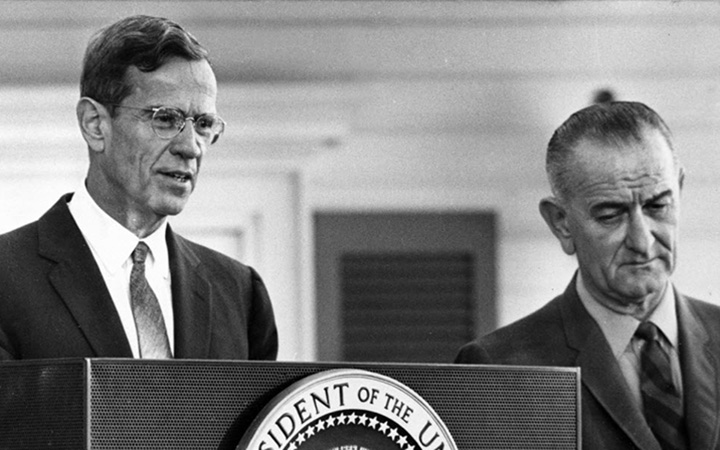
\includegraphics[height=0.75\textheight]{lbj-fed.jpg}
\end{figure}

\end{frame}
 
 %------------------------------------------------

\begin{frame}{Arms Sales}

\begin{figure}[htbp]
		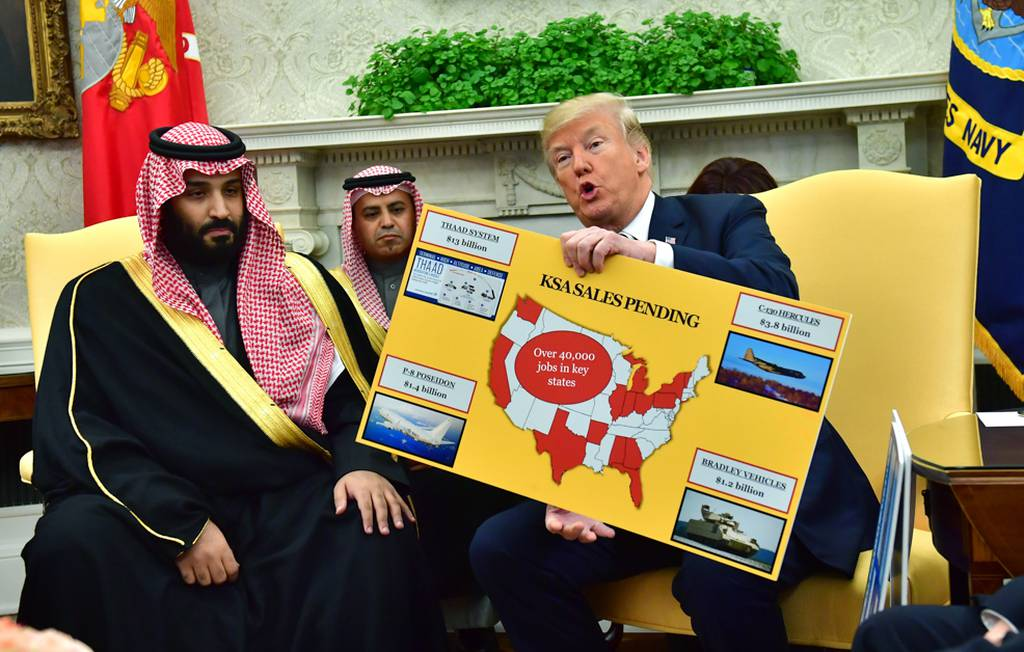
\includegraphics[width=0.75\textwidth]{trump-sales.jpg}
\end{figure}

\end{frame}
 
 %------------------------------------------------

\begin{frame}{My Argument in Brief}

\begin{enumerate}
\item U.S. political budget cycles increase trade.  
\pause 
\item Defense contracting has a critical role in budget cycles.
\pause 
\item Contracting cycles lead to arms exports, especially to allies. 
\pause
\item \textbf{Outcome}: U.S. imports increase, and allies receive more U.S. exports through arms. 
\end{enumerate}

\end{frame}


 %------------------------------------------------

\begin{frame}{The Contribution}


International security consequences of political budget cycles.  
\pause 
\begin{enumerate}
\item Most prior research focuses on presence and domestic consequences of cycles (e.g. Nordhaus 1975; Tufte 1978; Rogoff 1987). 
\pause 
\item Some work on international consequences, mostly in economic growth and finance: (e.g. Thompson and Zuk 1983; Ito 1991; Foerster and Schmitz 1997)
\pause 
\item Identifying general trade cycles makes a marginal contribution. 
\end{enumerate}

\end{frame}


%------------------------------------------------

\begin{frame}{Outline}

\pause
\begin{enumerate}
\item Argument: Budget Cycles, Defense Contracting, Arms Transfers, and Trade. 
\pause
\item Results: Electoral Trade Cycles. 
\pause
\item Results: Defense Contracting and Arms Trade Cycles.  
\end{enumerate}


\end{frame}
 

%------------------------------------------------

\section{Argument} 

%-----------------------------------------------

\begin{frame}{Political Budget Cycles}

In order to win elections:
\pause 
\begin{enumerate} 
\item Leaders use fiscal and monetary policy to increase economic growth. 
\pause 
\item Also employ targeted policies (Conconi et al. 2017; Ahlquist 2010, Philips 2020). 
\end{enumerate}


\end{frame} 

%-----------------------------------------------

\begin{frame}{Economic Consequences of Budget Cycles}

\pause 
\begin{enumerate} 
\item Economic expansion increases domestic consumption, pulling in imports.  
\pause 
\item Price effects of monetary expansion increase exports. Likely weaker effect (Clark and Hallerberg 2000). 
\pause
\item Imports from all other countries rise. Exports increase somewhat. 
\end{enumerate}


\end{frame} 

%-----------------------------------------------

\begin{frame}{Defense Contracting and Arms Exports}

\pause 
\begin{enumerate} 
\item Presidents control contract allocation.  
\pause 
\item Use this for targeted stimulus (Mayer 1995; DeRouen Jr and Heo 2000).
\pause
\item Creates additional defense goods.
\pause
\item Some defense goods will be exported.
\end{enumerate}


\end{frame} 

%-----------------------------------------------

\begin{frame}{Arms Exports to Allies}

\pause 
\begin{enumerate} 
\item Allies provide a market for additional defense goods.
\pause 
\item Result of common security interests, defense industry integration. 
\pause
\item Exports double as a commitment signal for U.S. leaders (Yarhi-Milo et al 2018). 
\pause
\item Allies gain security and establish a cooperative reputation.
\end{enumerate}


\end{frame} 

%-----------------------------------------------

\begin{frame}[fragile]{Argument Summary}

\begin{figure}[htpb]
\adjustbox{scale = .65}{
\begin{tikzcd}[ampersand replacement=\&]
                                                                               \&             \&          \&  |[visible on=<2->, alias=Y]| \mbox{Trade Cycles}   \\
|[visible on=<1->]|  \mbox{Budget Cycles} \arrow[to = Y, visible on=<2->, bend left = 15] \arrow[visible on=<3->, r]  \& |[visible on=<3->]| \mbox{Defense Contracting} \arrow[ visible on=<4->, r] \& |[visible on=<4->]| \mbox{Arms Production} \arrow[visible on=<5->, r] \& |[visible on=<5->]| \mbox{Arms to Allies} \arrow[visible on=<6->, u]  
\end{tikzcd}
}
\end{figure}

\end{frame} 


%-----------------------------------------------

\begin{frame}[fragile]{Hypotheses}

\begin{quote}
\textsc{Trade Cycles Hypothesis}: As time to a presidential election decreases, U.S. imports will increase, and exports to allies will increase more than exports to non-allies.
\end{quote}
\pause

\vspace{5mm}

\begin{quote}
\textsc{Arms Exports Hypothesis}: As time to a presidential election decreases, U.S. arms exports to allies will increase.
\end{quote}

\end{frame}

%-----------------------------------------------

%------------------------------------------------

\section{Electoral Trade Cycles} 

%-----------------------------------------------

\begin{frame}{Research Design}

\pause
Analyze changes in US trade with all other states, 1951 to 2014. 
\pause
\begin{enumerate}
\item Outcome: Changes in log exports and imports.
\pause
\item Independent Variables: Dummy indicator of defense alliance, years to presidential election, interaction. 
\pause 
\item Estimator: Robust regression. 
\pause 
\item Adjust for gravity model factors, security threats, common interests, presidential partisanship.
\end{enumerate} 

\end{frame} 

%-----------------------------------------------

\begin{frame}{Electoral Trade Cycles}

\begin{figure}[htbp]
	\centering
		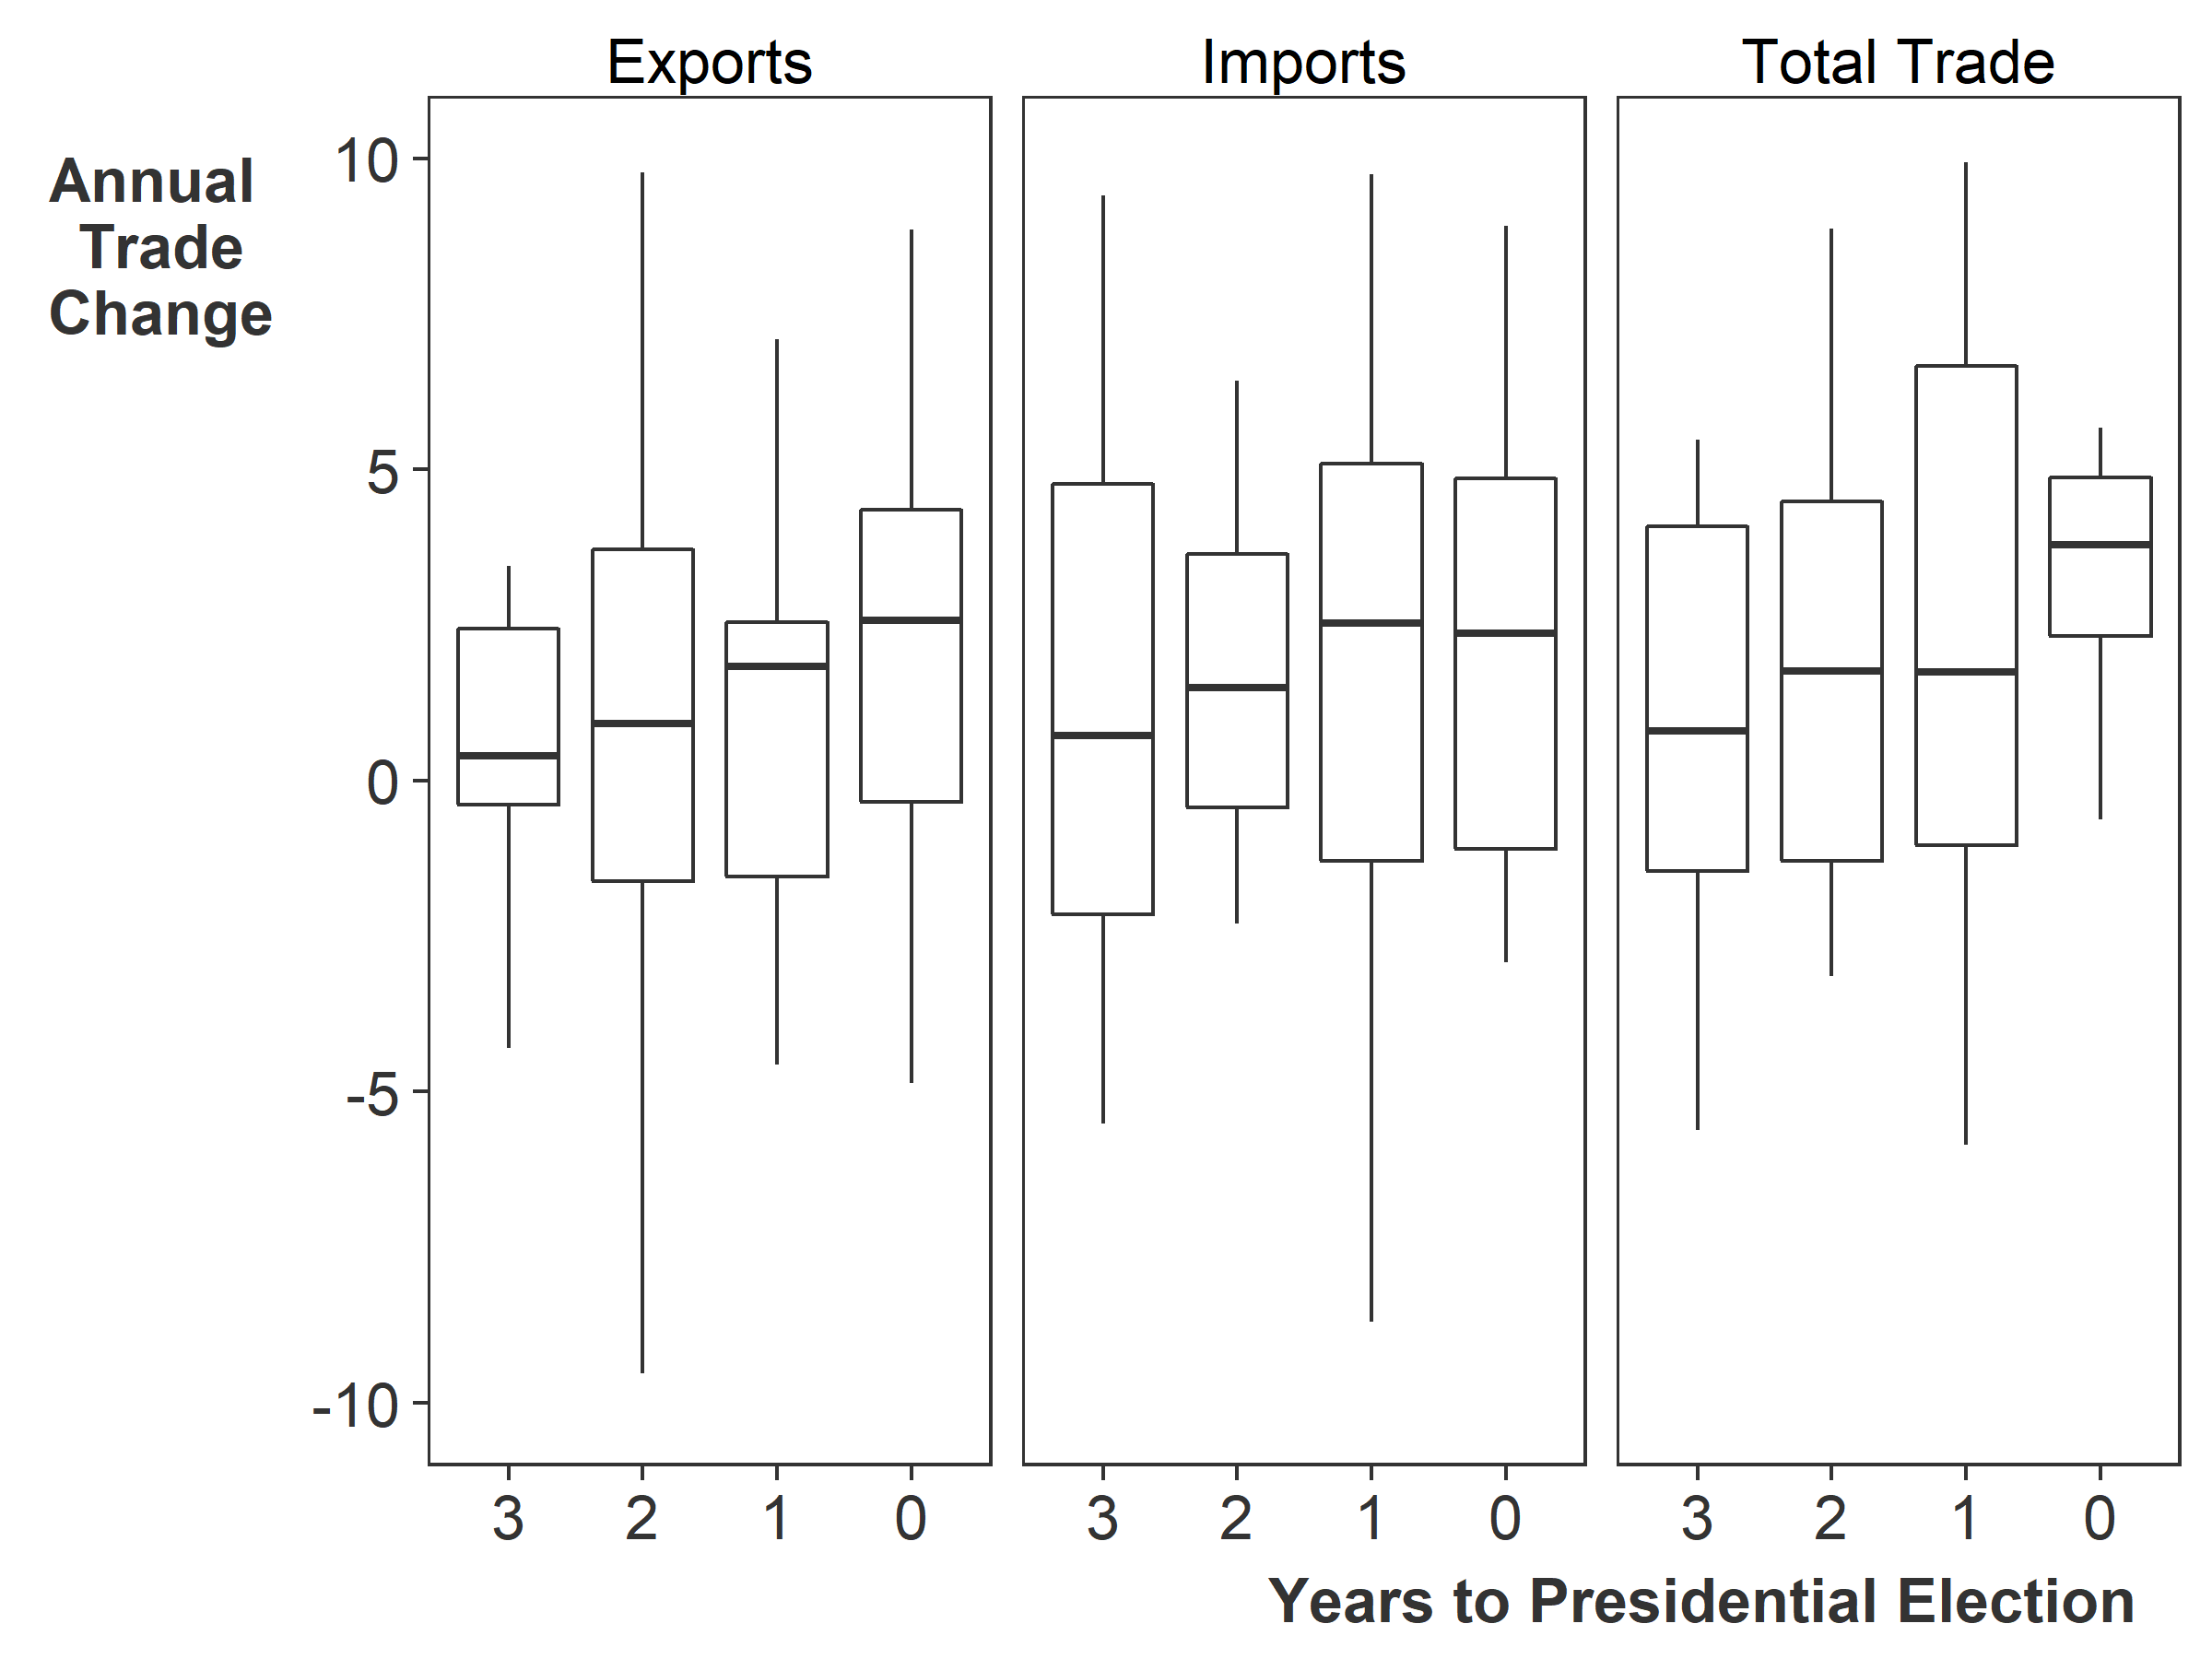
\includegraphics[height=.9\textheight]{us-trade-cycles.png}
\end{figure}


\end{frame} 


%-----------------------------------------------

\begin{frame}{Alliances and Trade Regression Results}

\pause
\begin{figure}[htbp]
	\centering
		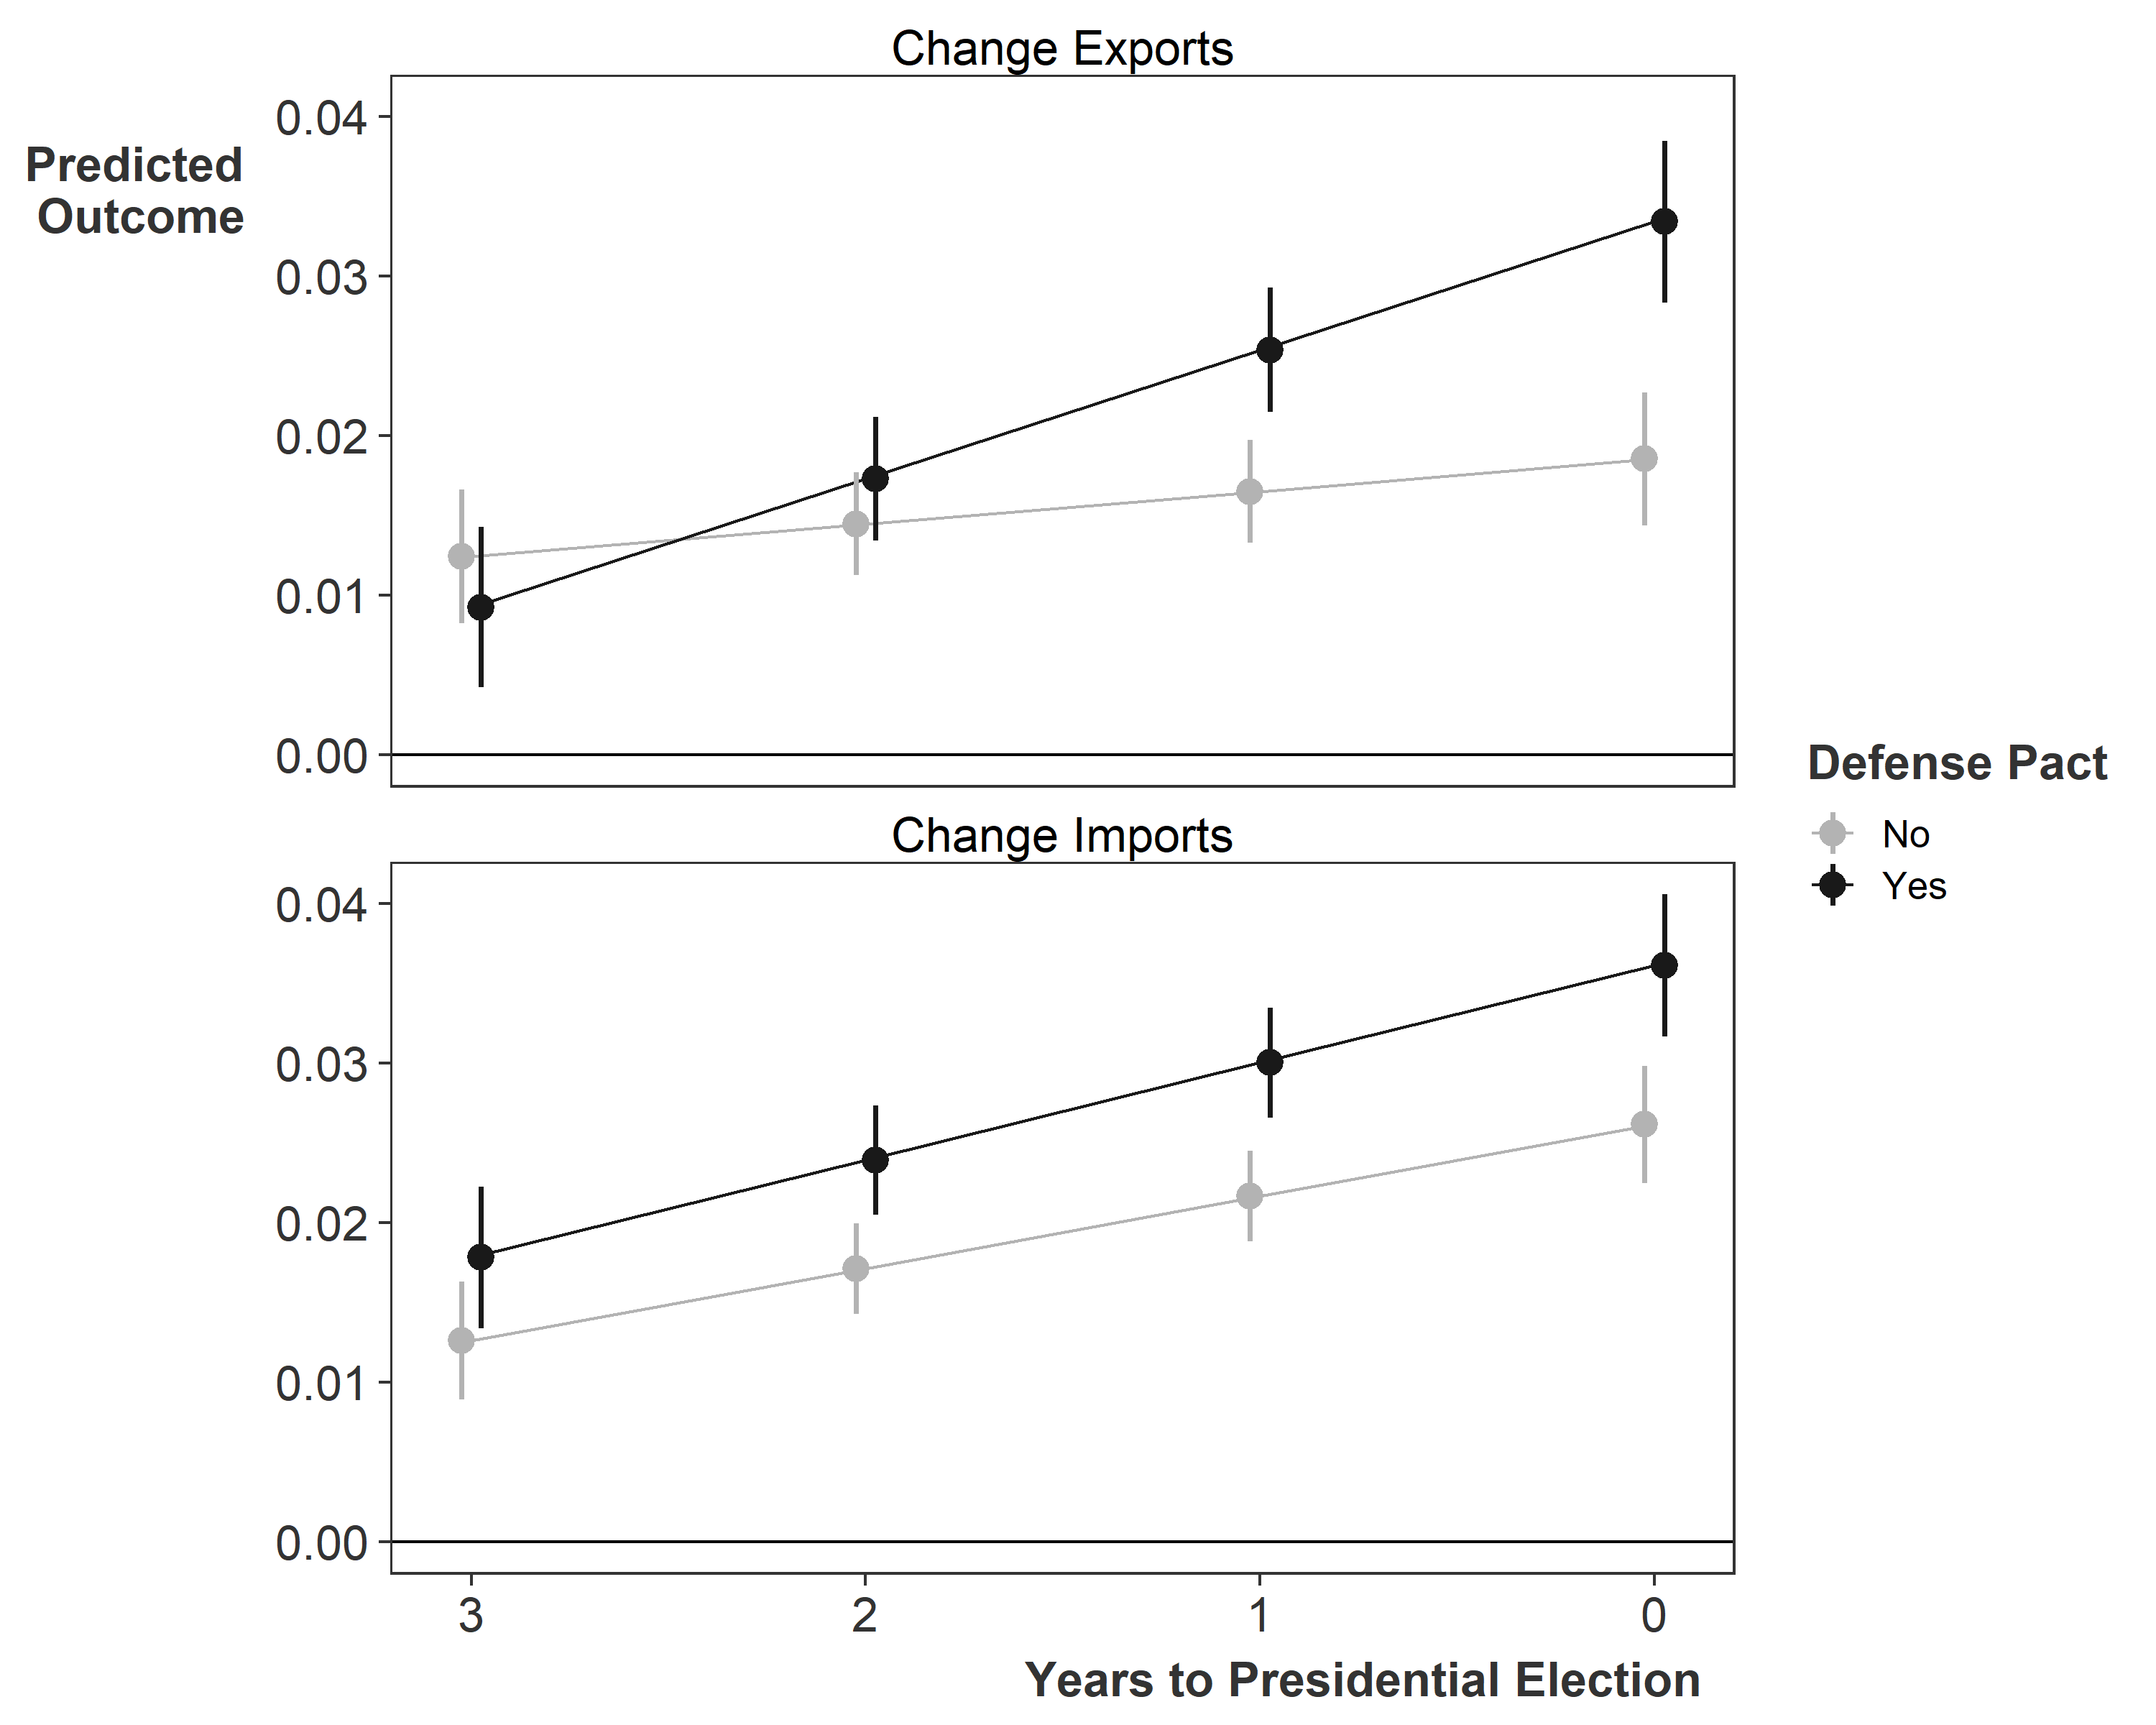
\includegraphics[height=.9\textheight]{us-elec-pred-exim.png}
\end{figure}

\end{frame} 



%------------------------------------------------

\section{Arms Export Cycles} 

%-----------------------------------------------

\begin{frame}{Research Design}

\pause
Analyze US arms exports to all other states, 1951 to 2014. 
\pause
\begin{enumerate}
\item Outcome: Log Arms Transfers (SIPRI), non-zero values. 
\pause
\item Independent Variables: Dummy indicator of defense alliance, years to presidential election, interaction. 
\pause 
\item Estimator: Linear regression (OLS) with hurdle. 
\pause 
\item Adjust for trade model controls, lagged arms transfers, and non-zero arms transfer probability.
\end{enumerate} 

\end{frame} 

%-------------------------------------------------

\begin{frame}{Arms Exports, Alliances, and Elections}

\begin{figure}[htbp]
	\centering
		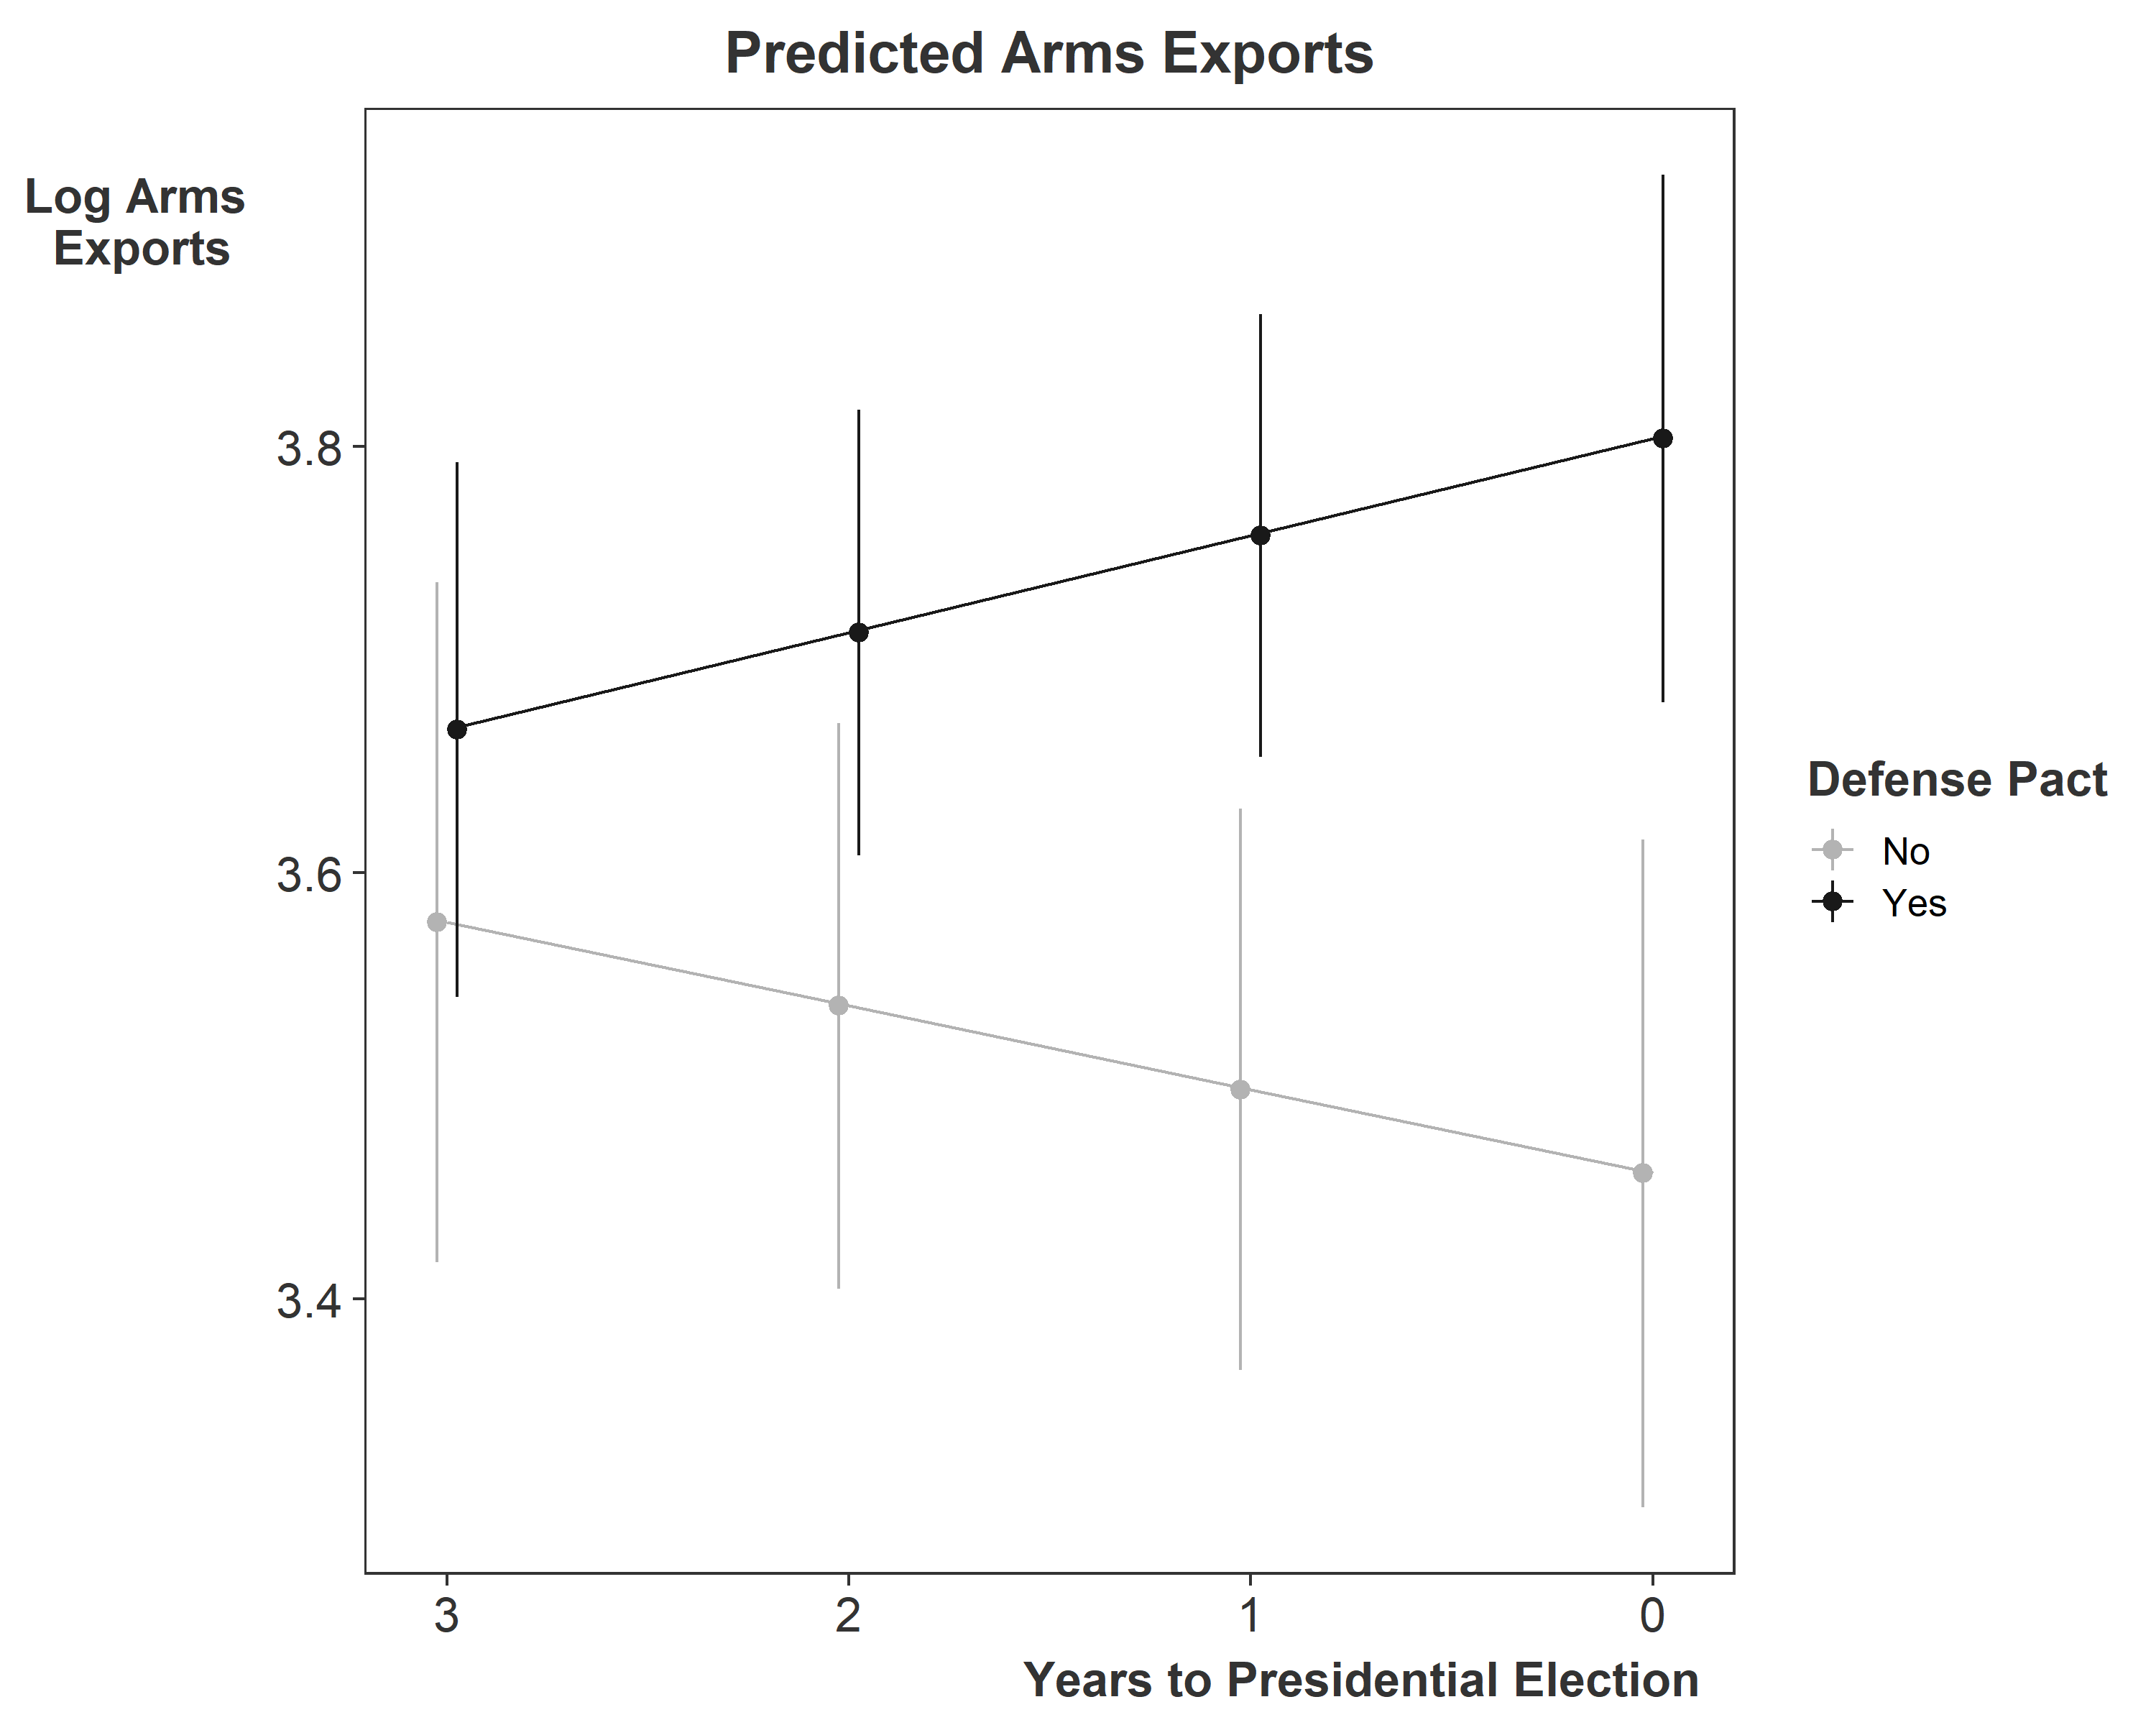
\includegraphics[height=.90\textheight]{us-arms-pred.png}
\end{figure}

\end{frame}


%------------------------------------------------

\section{Defense Contracting Cycles} 

%-----------------------------------------------


\begin{frame}{Defense Contracting Cycles: 2000-2020}

\begin{figure}[htbp]
	\centering
		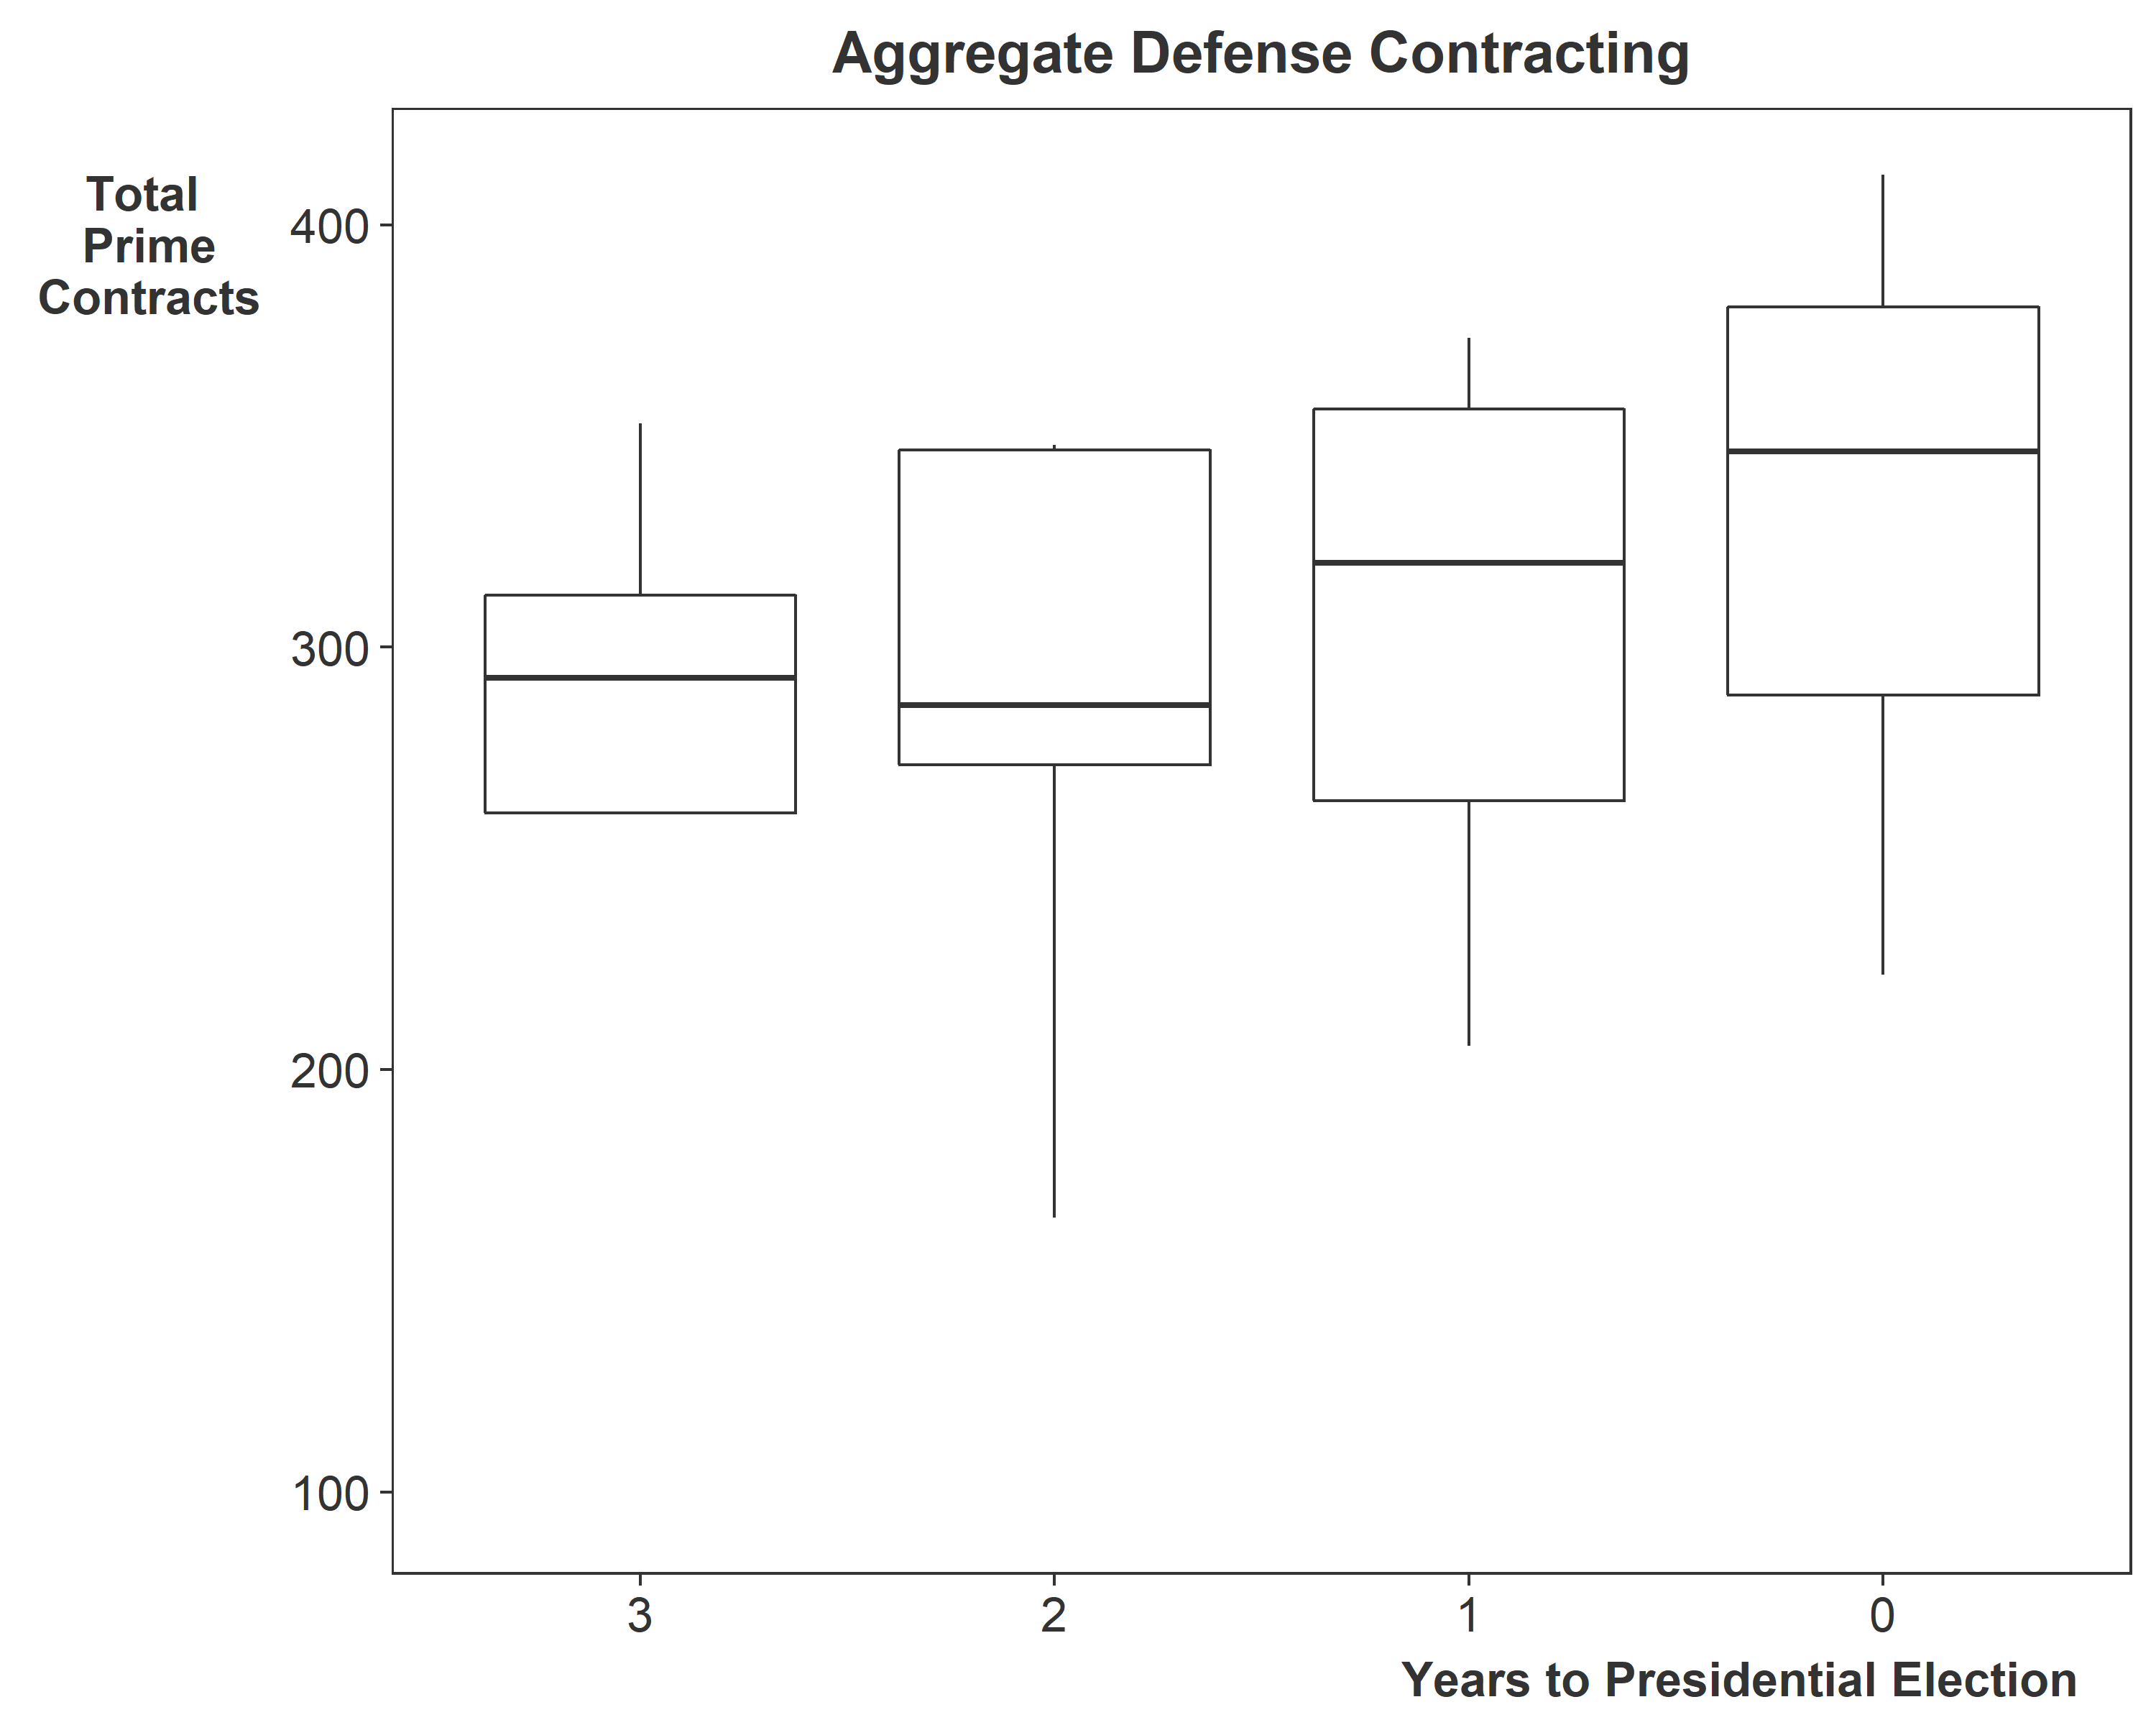
\includegraphics[height=.90\textheight]{contract-cycles.png}
\end{figure}


\end{frame}



%-----------------------------------------------


%------------------------------------------------

\section{Discussion and Conclusion} 

%-----------------------------------------------


\begin{frame}[standout]

U.S. political budget cycles expand international trade, especially arms exports to allies.  

\end{frame}


%------------------------------------------------
\begin{frame}{Discussion}

Some limitations. 

\pause
\begin{enumerate}
\item Collecting more detailed trade and arms data. 
\pause
\item Generalizing beyond the United States. 
\end{enumerate} 

\end{frame}


%%------------------------------------------------
\begin{frame}{My Research Agenda: Alliance Politics and Political Economy of Security}

\begin{columns}

% Major powers
\begin{column}{0.5\textwidth}
\textbf{Alliance Politics}
\begin{enumerate} 
\item Alliances and Military Spending: \textit{International Studies Quarterly}, \textit{Research \& Politics} and  \textit{Security Studies}.
\item Economic Benefits of US Alliances. 
\item Democratic Alliance Durability.
\end{enumerate} 
\end{column}


\begin{column}{0.5\textwidth}
\textbf{Civil Conflict}
\begin{enumerate}
\item U.S. Foreign Terrorist Organization (FTO) List and Terrorist Attacks 
\item Conflict Management Institutions and FDI in Post-Conflict States
\item Media and Support for Militant Right-Wing Extremism in the U.S.
\end{enumerate} 
\end{column}


\end{columns}
 

\end{frame}



%------------------------------------------------
\begin{frame}{Teaching Interests}

At the Bush School in DC, I could offer courses in: 
\pause 
\begin{enumerate}
\item Global Economy
\pause
\item Political Economy of Security
\pause
\item NATO and European Security
\pause 
\item Research Methods
\pause
\item Foreign Policy Mistakes
\end{enumerate} 

\end{frame}

%-----------------------------------------------


%------------------------------------------------

\begin{frame}[standout]

Thank you! 

jkalley@virginia.edu

\end{frame}

%-----------------------------------------------

\appendix 

%-----------------------------------------------


%-----------------------------------------------

\begin{frame}{Interaction Terms: Alliances and Trade}

\begin{figure}[htbp]
	\centering
		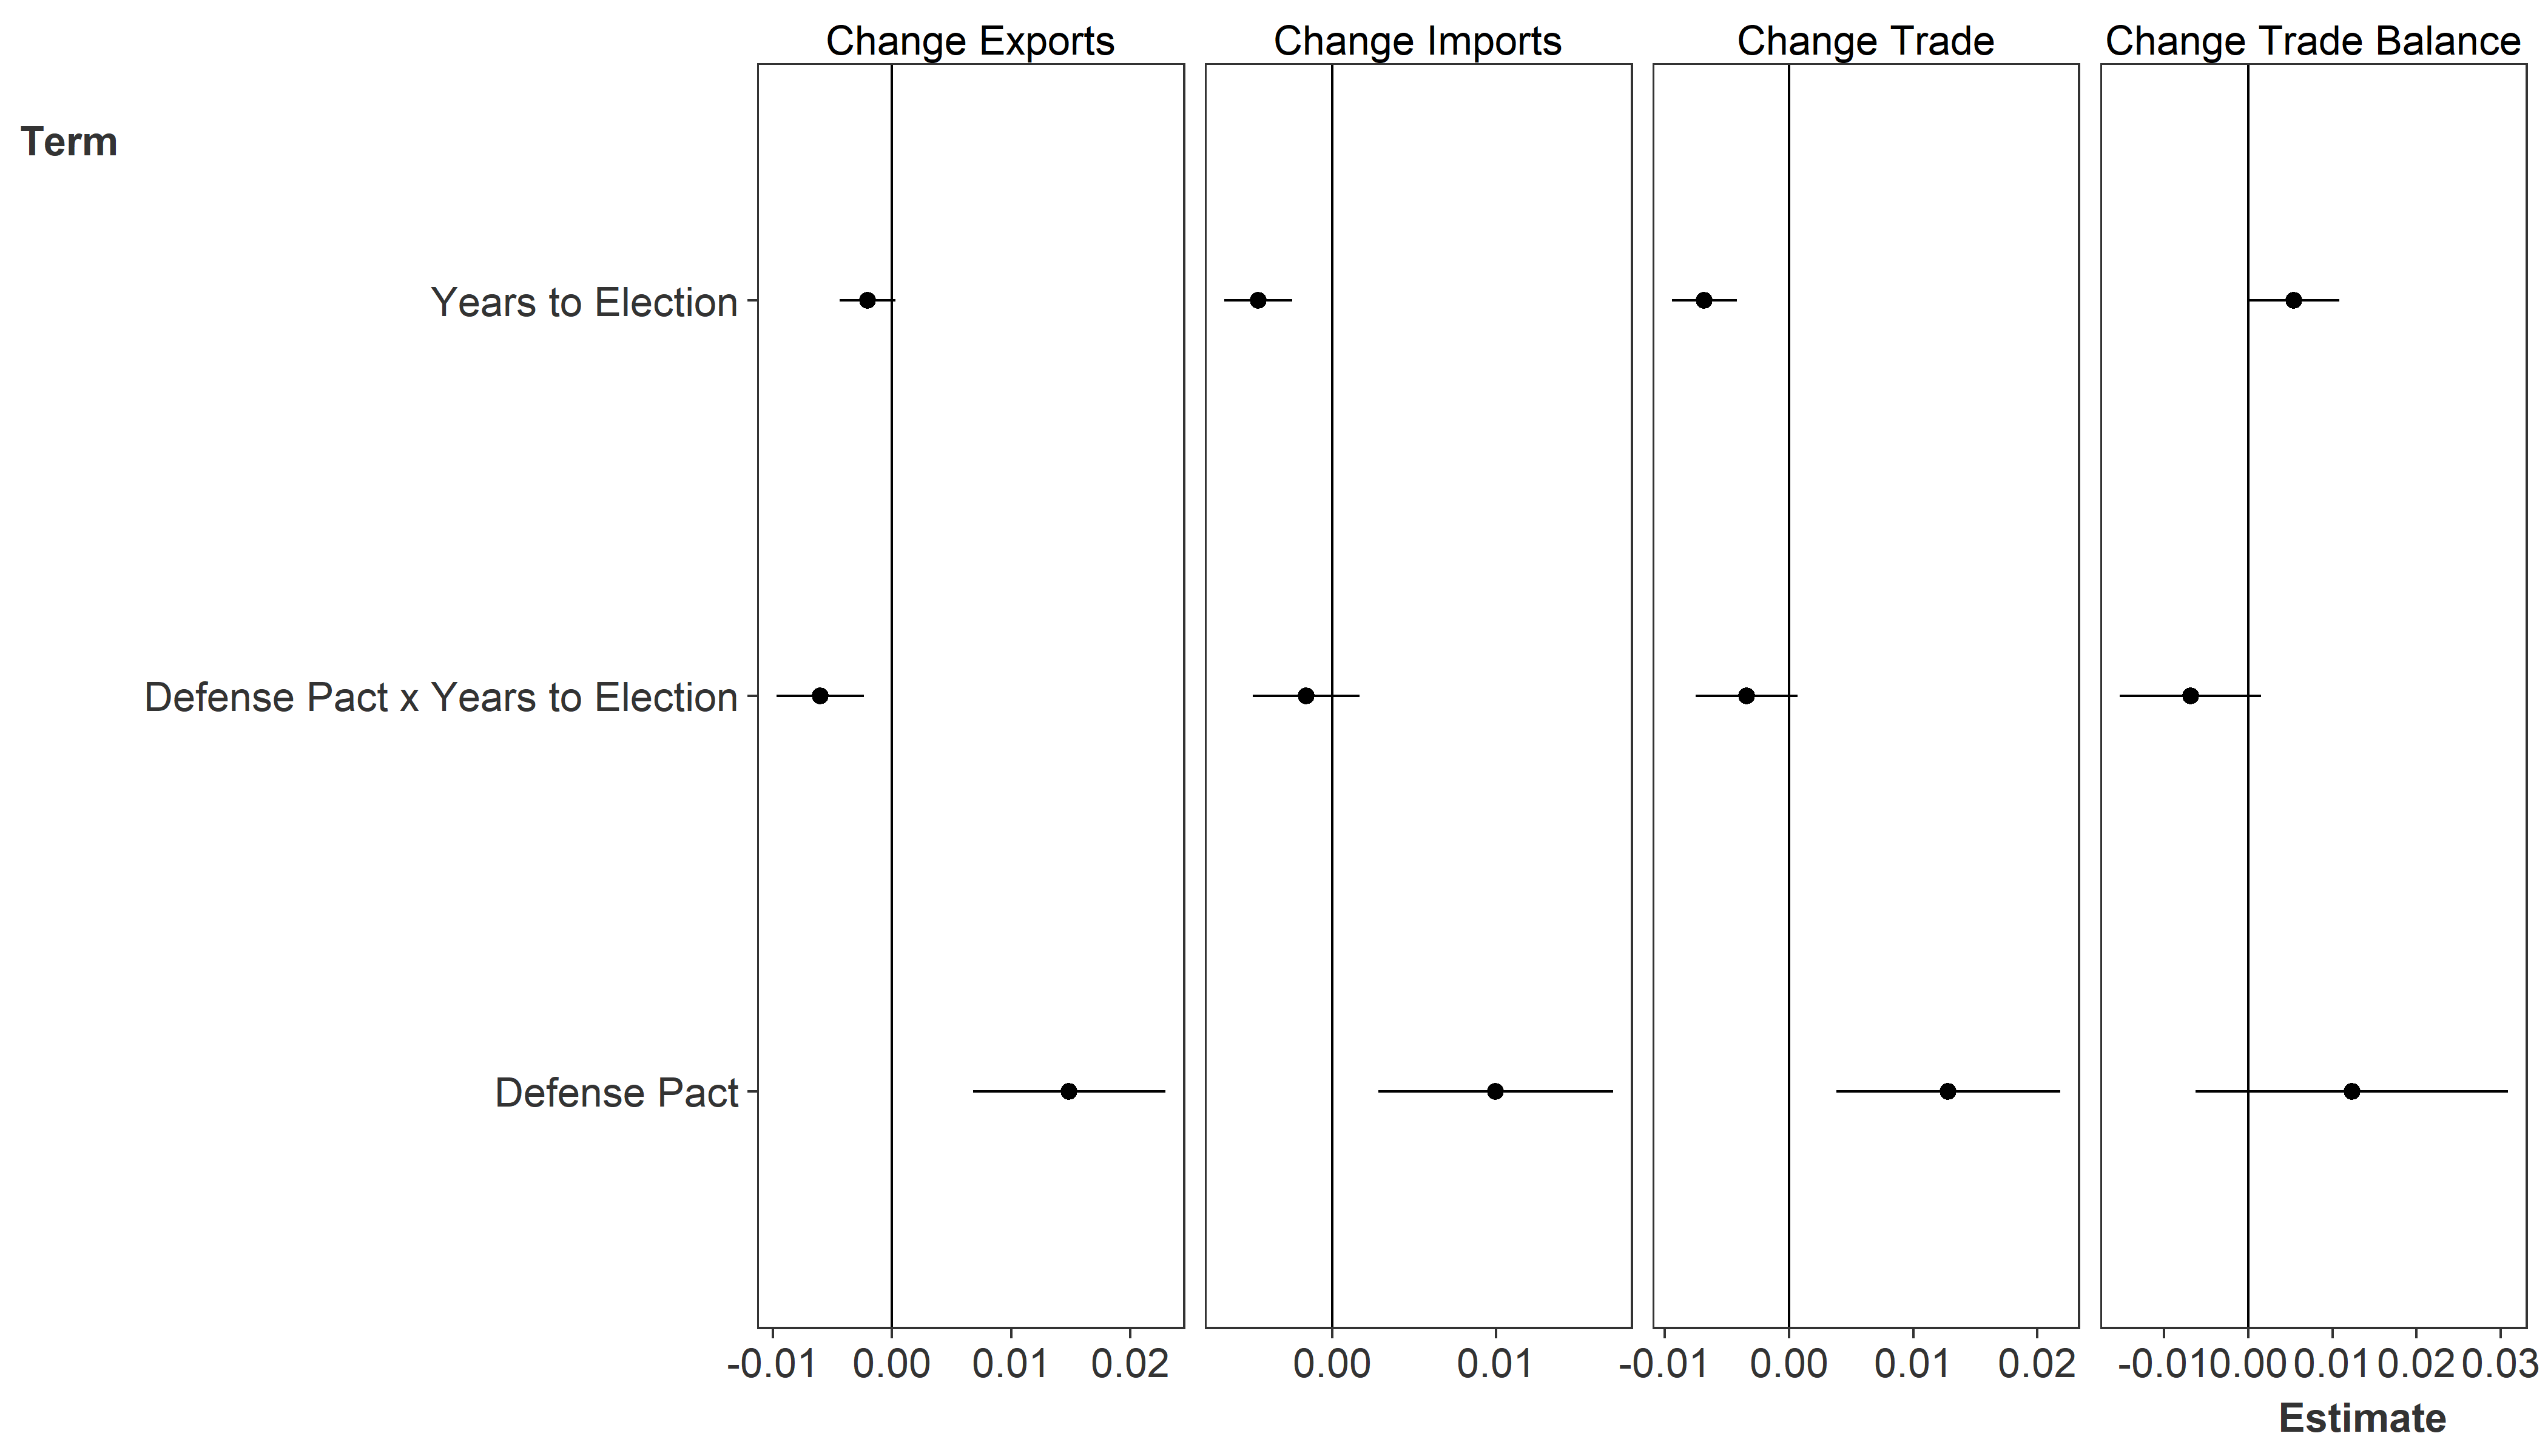
\includegraphics[width=.90\textwidth]{trade-inter-terms.png}
\end{figure}


\end{frame}


%-----------------------------------------------

\begin{frame}{Marginal Effects: Alliances and Trade}

\begin{figure}[htbp]
	\centering
		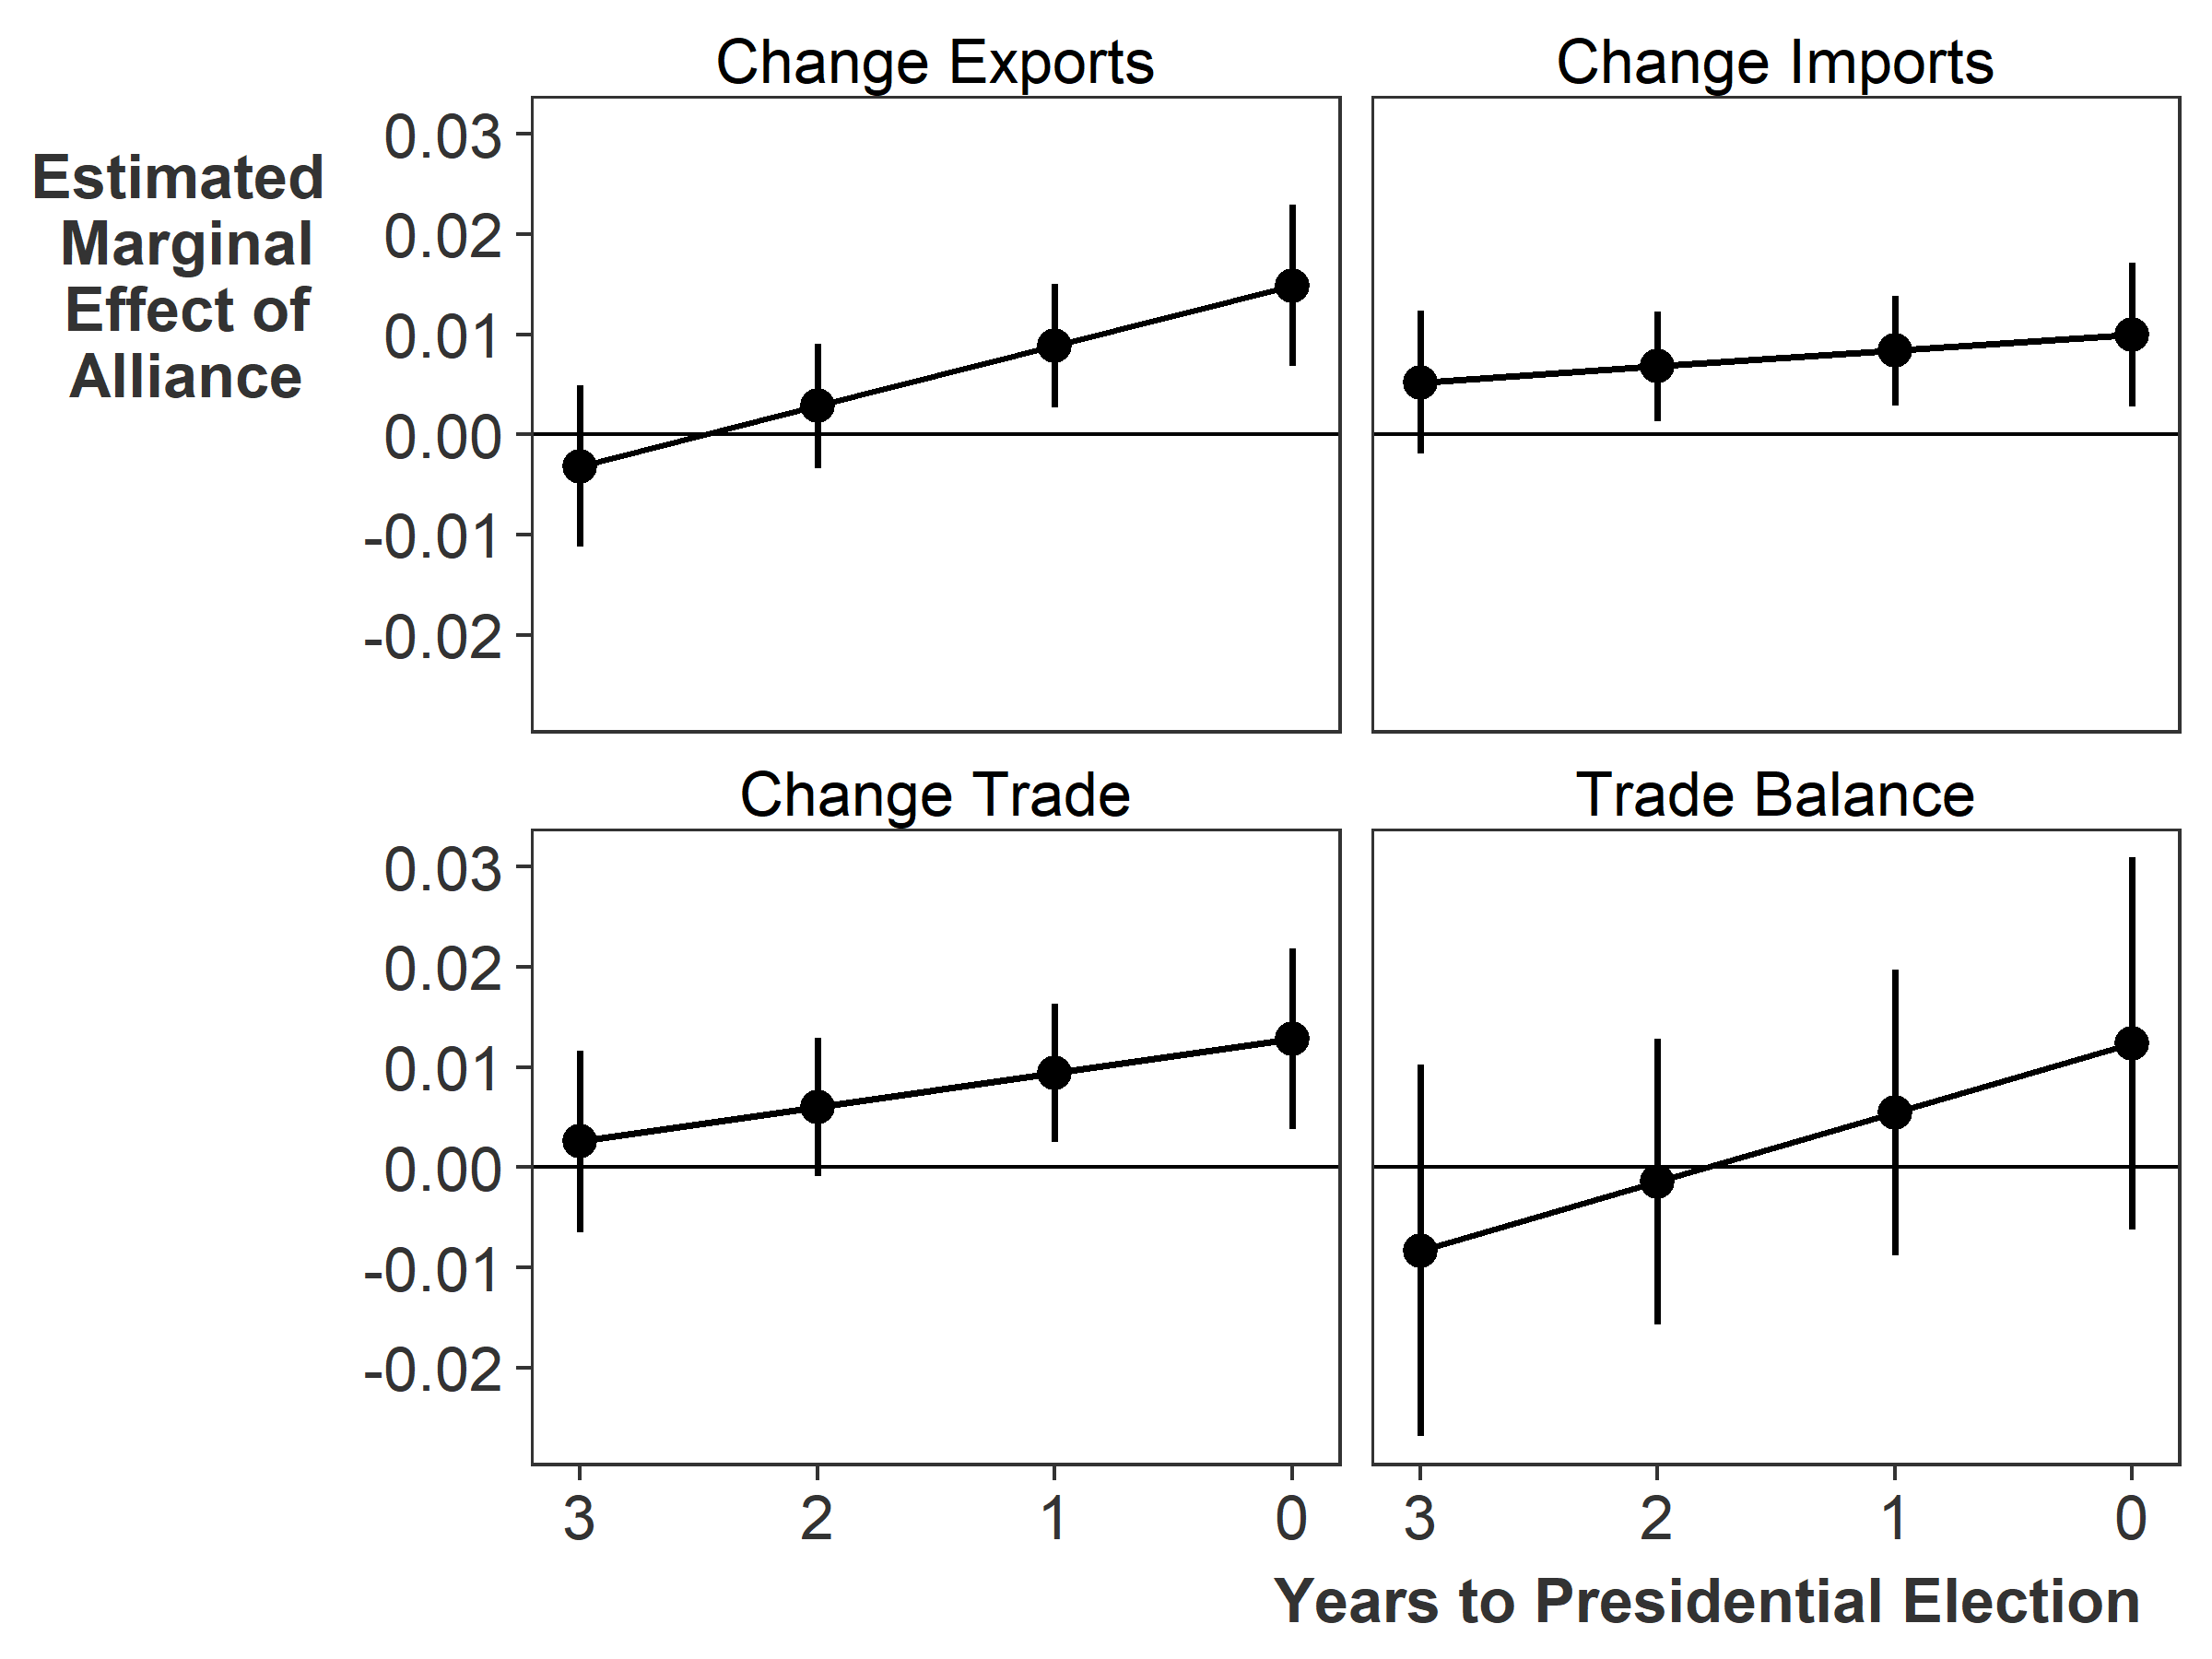
\includegraphics[height=.90\textheight]{us-defense-me.png}
\end{figure}


\end{frame}


%-----------------------------------------------

\begin{frame}{Net Trade Outcomes}

\begin{figure}[htbp]
	\centering
		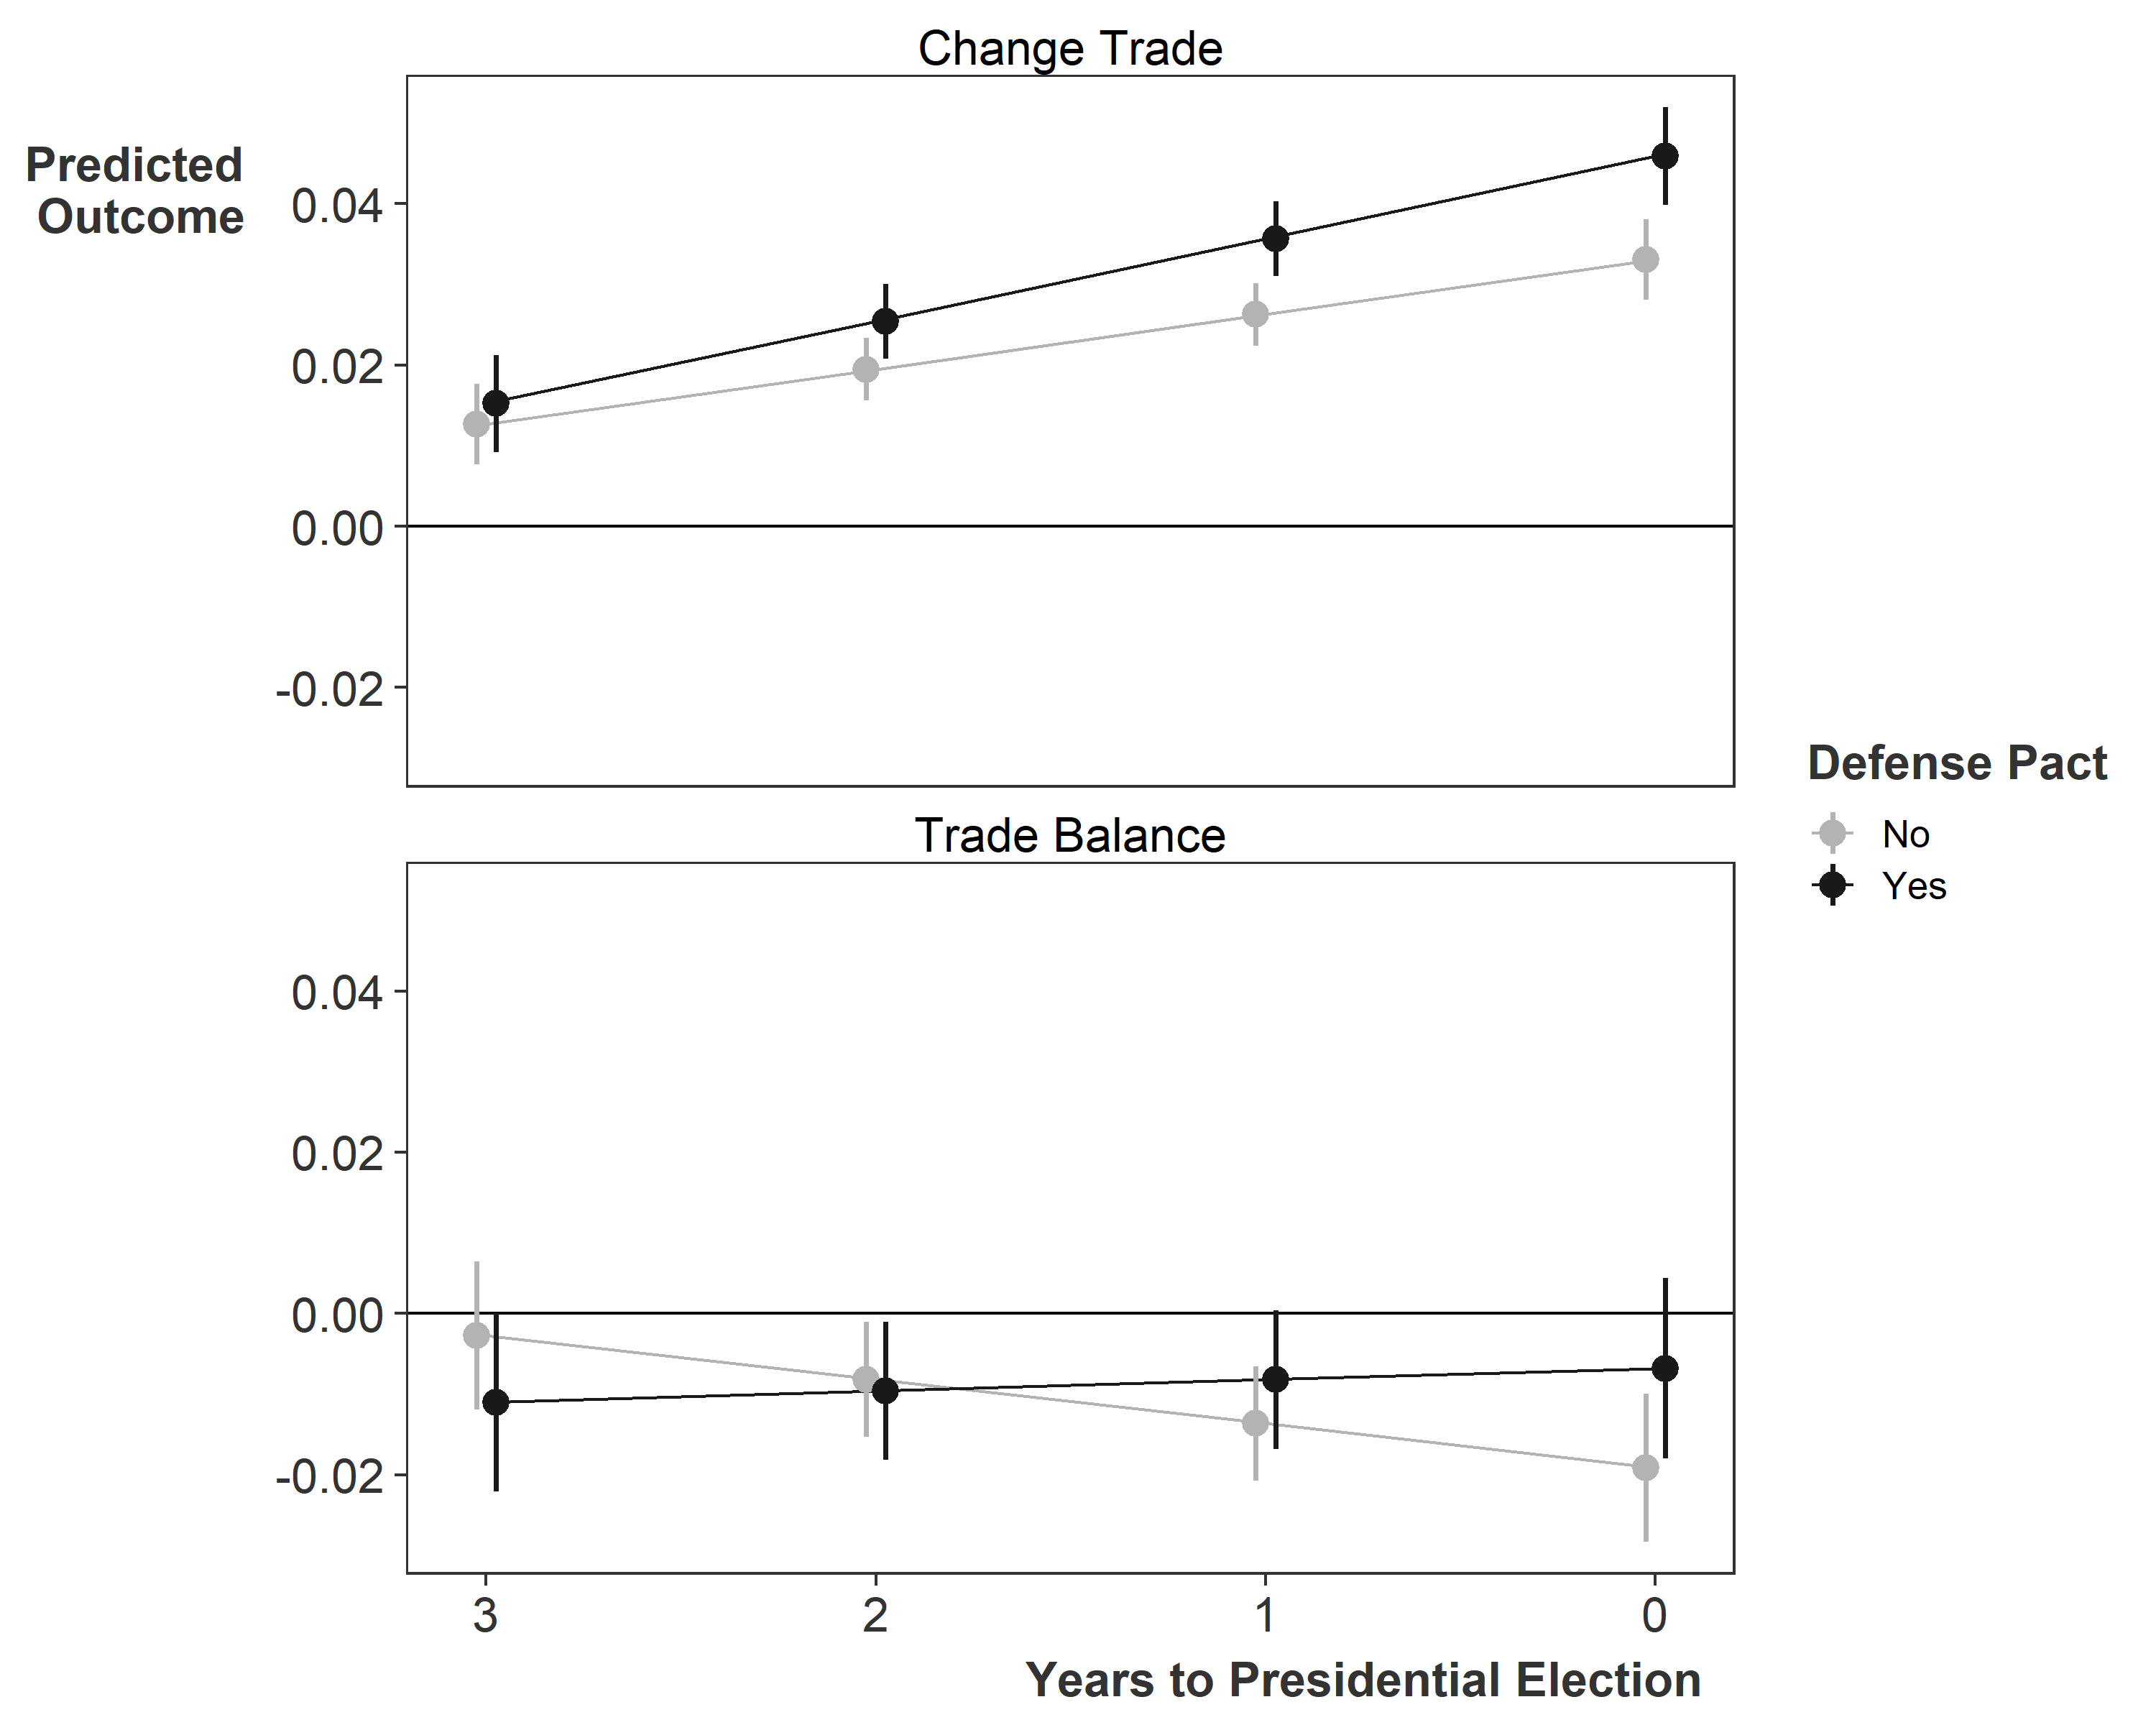
\includegraphics[height=.90\textheight]{us-elec-pred-net.png}
\end{figure}


\end{frame}



%-----------------------------------------------

\begin{frame}{Marginal Effects: Alliances and Arms Exports}

\begin{figure}[htbp]
	\centering
		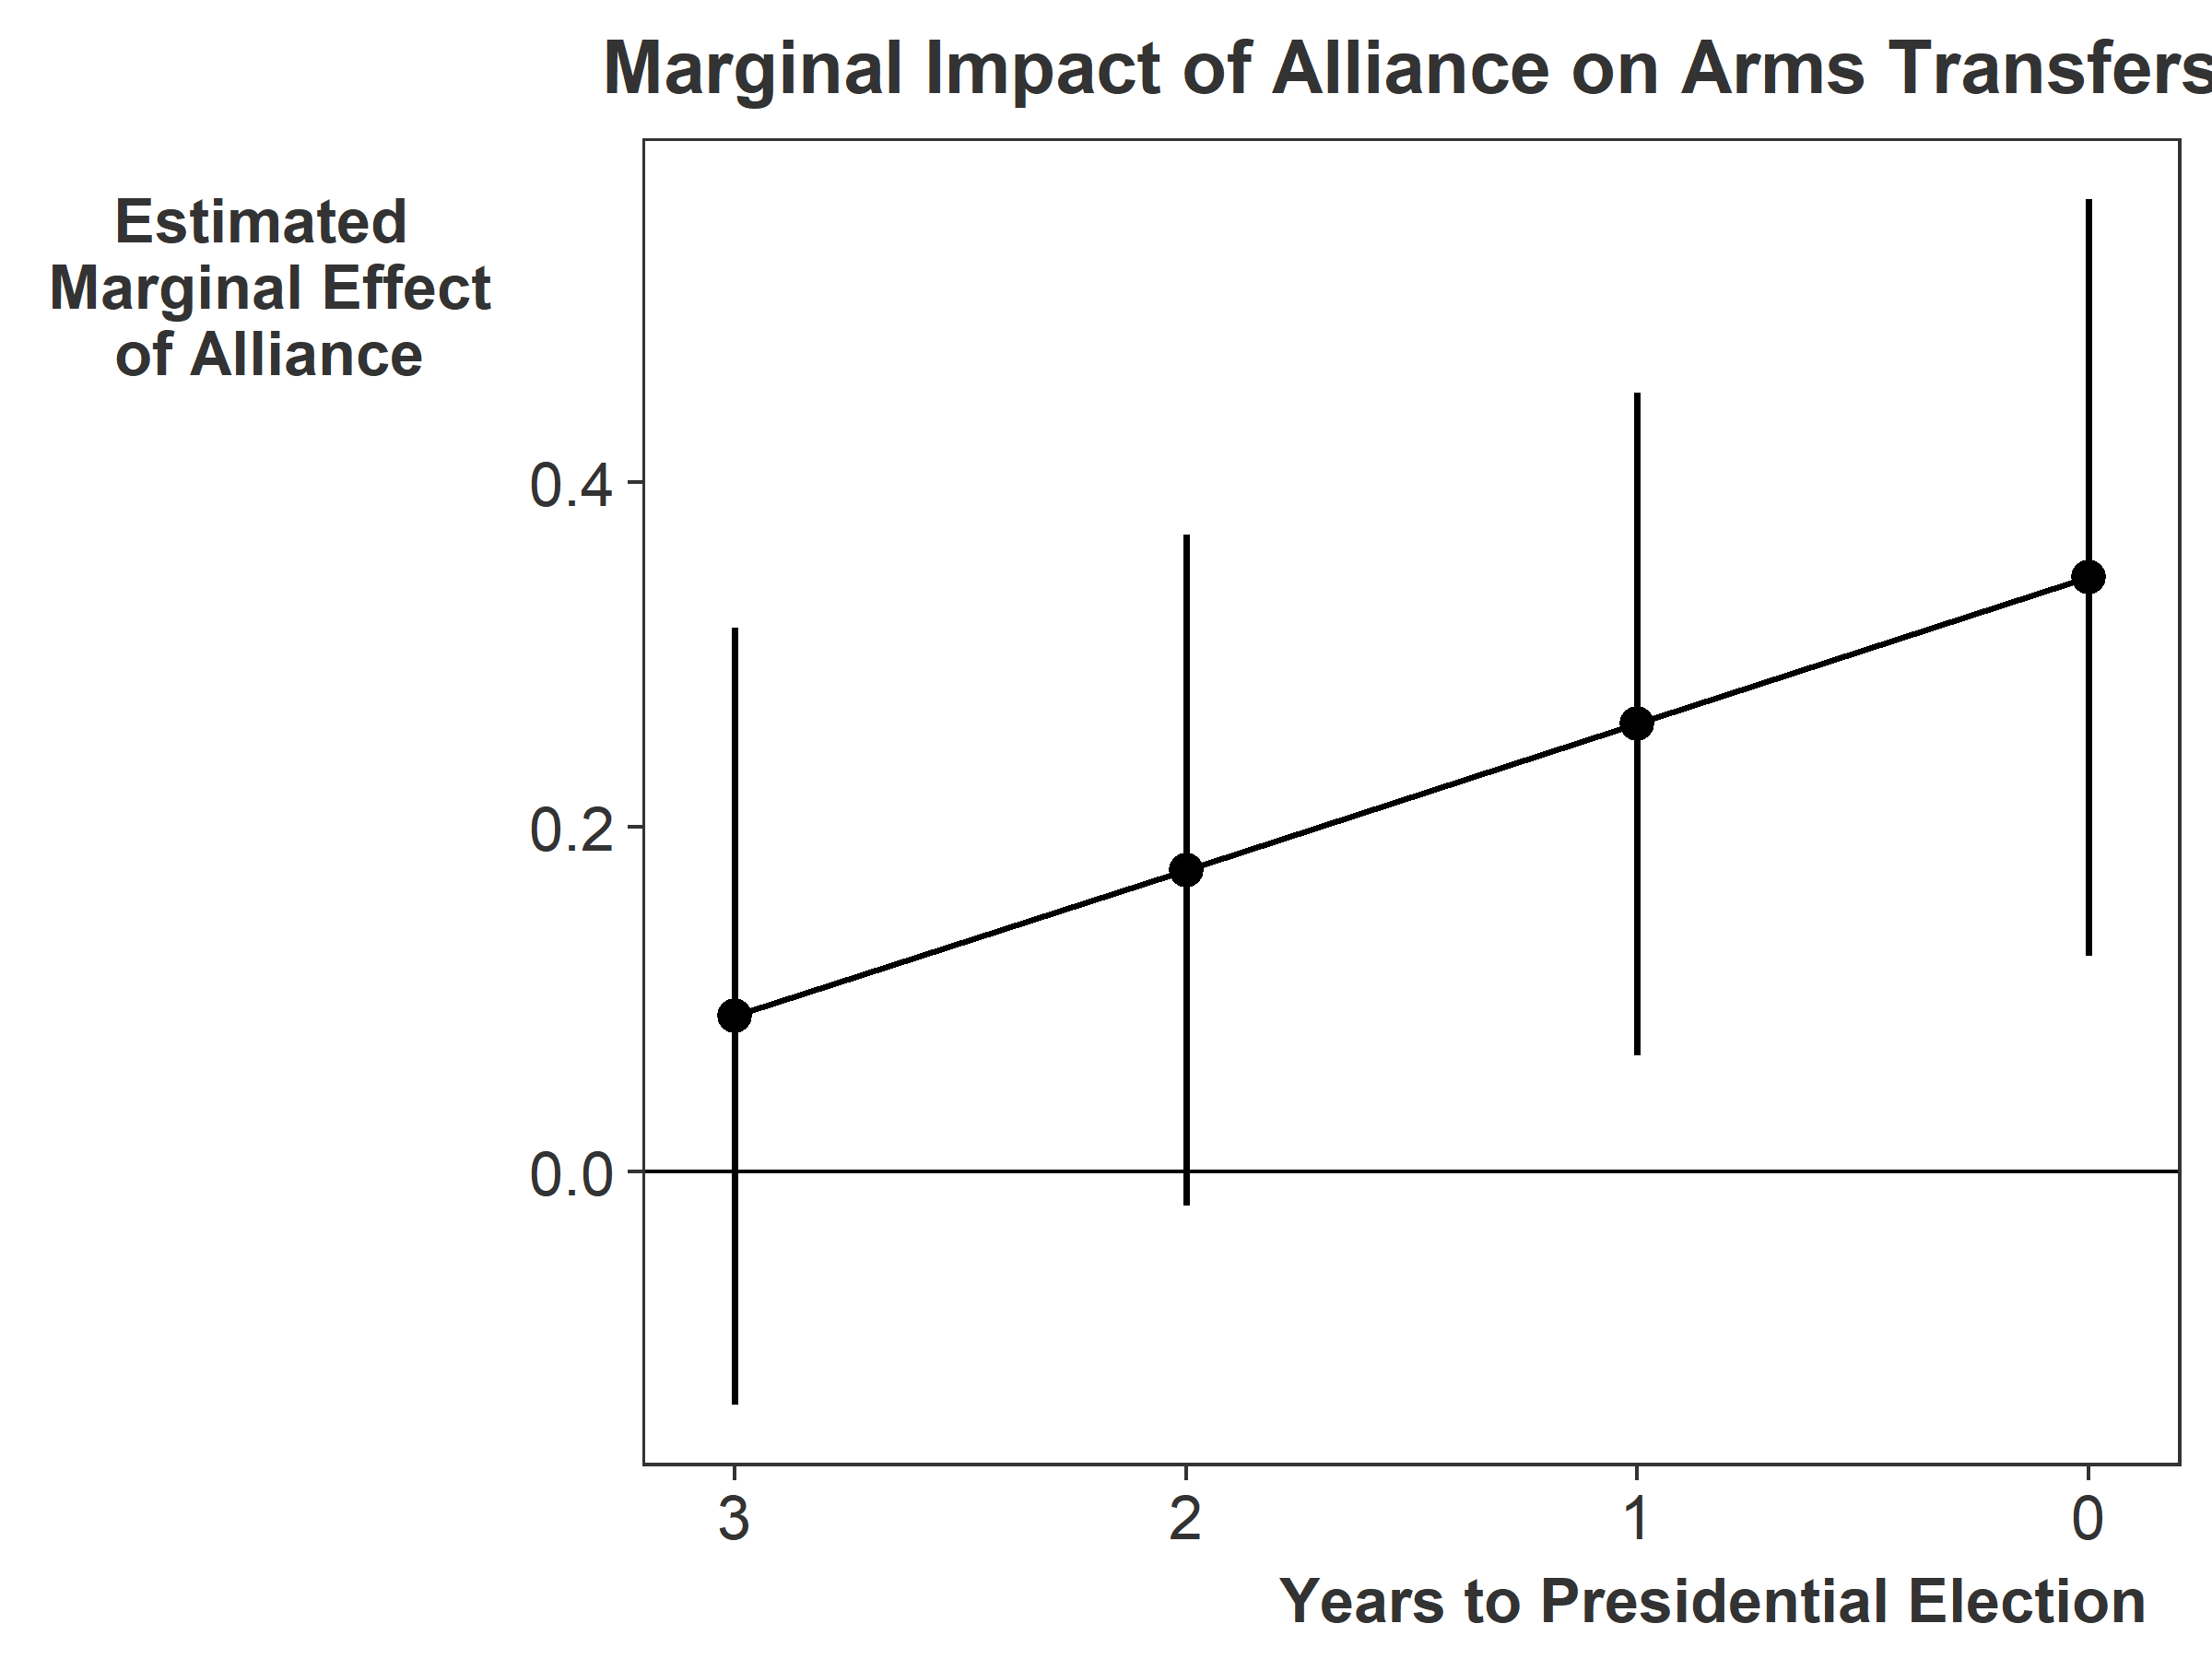
\includegraphics[height=.90\textheight]{us-defense-me-arms.png}
\end{figure}


\end{frame}

%-----------------------------------------------

\begin{frame}{Defense Contracting by Sector}

\begin{figure}[htbp]
	\centering
		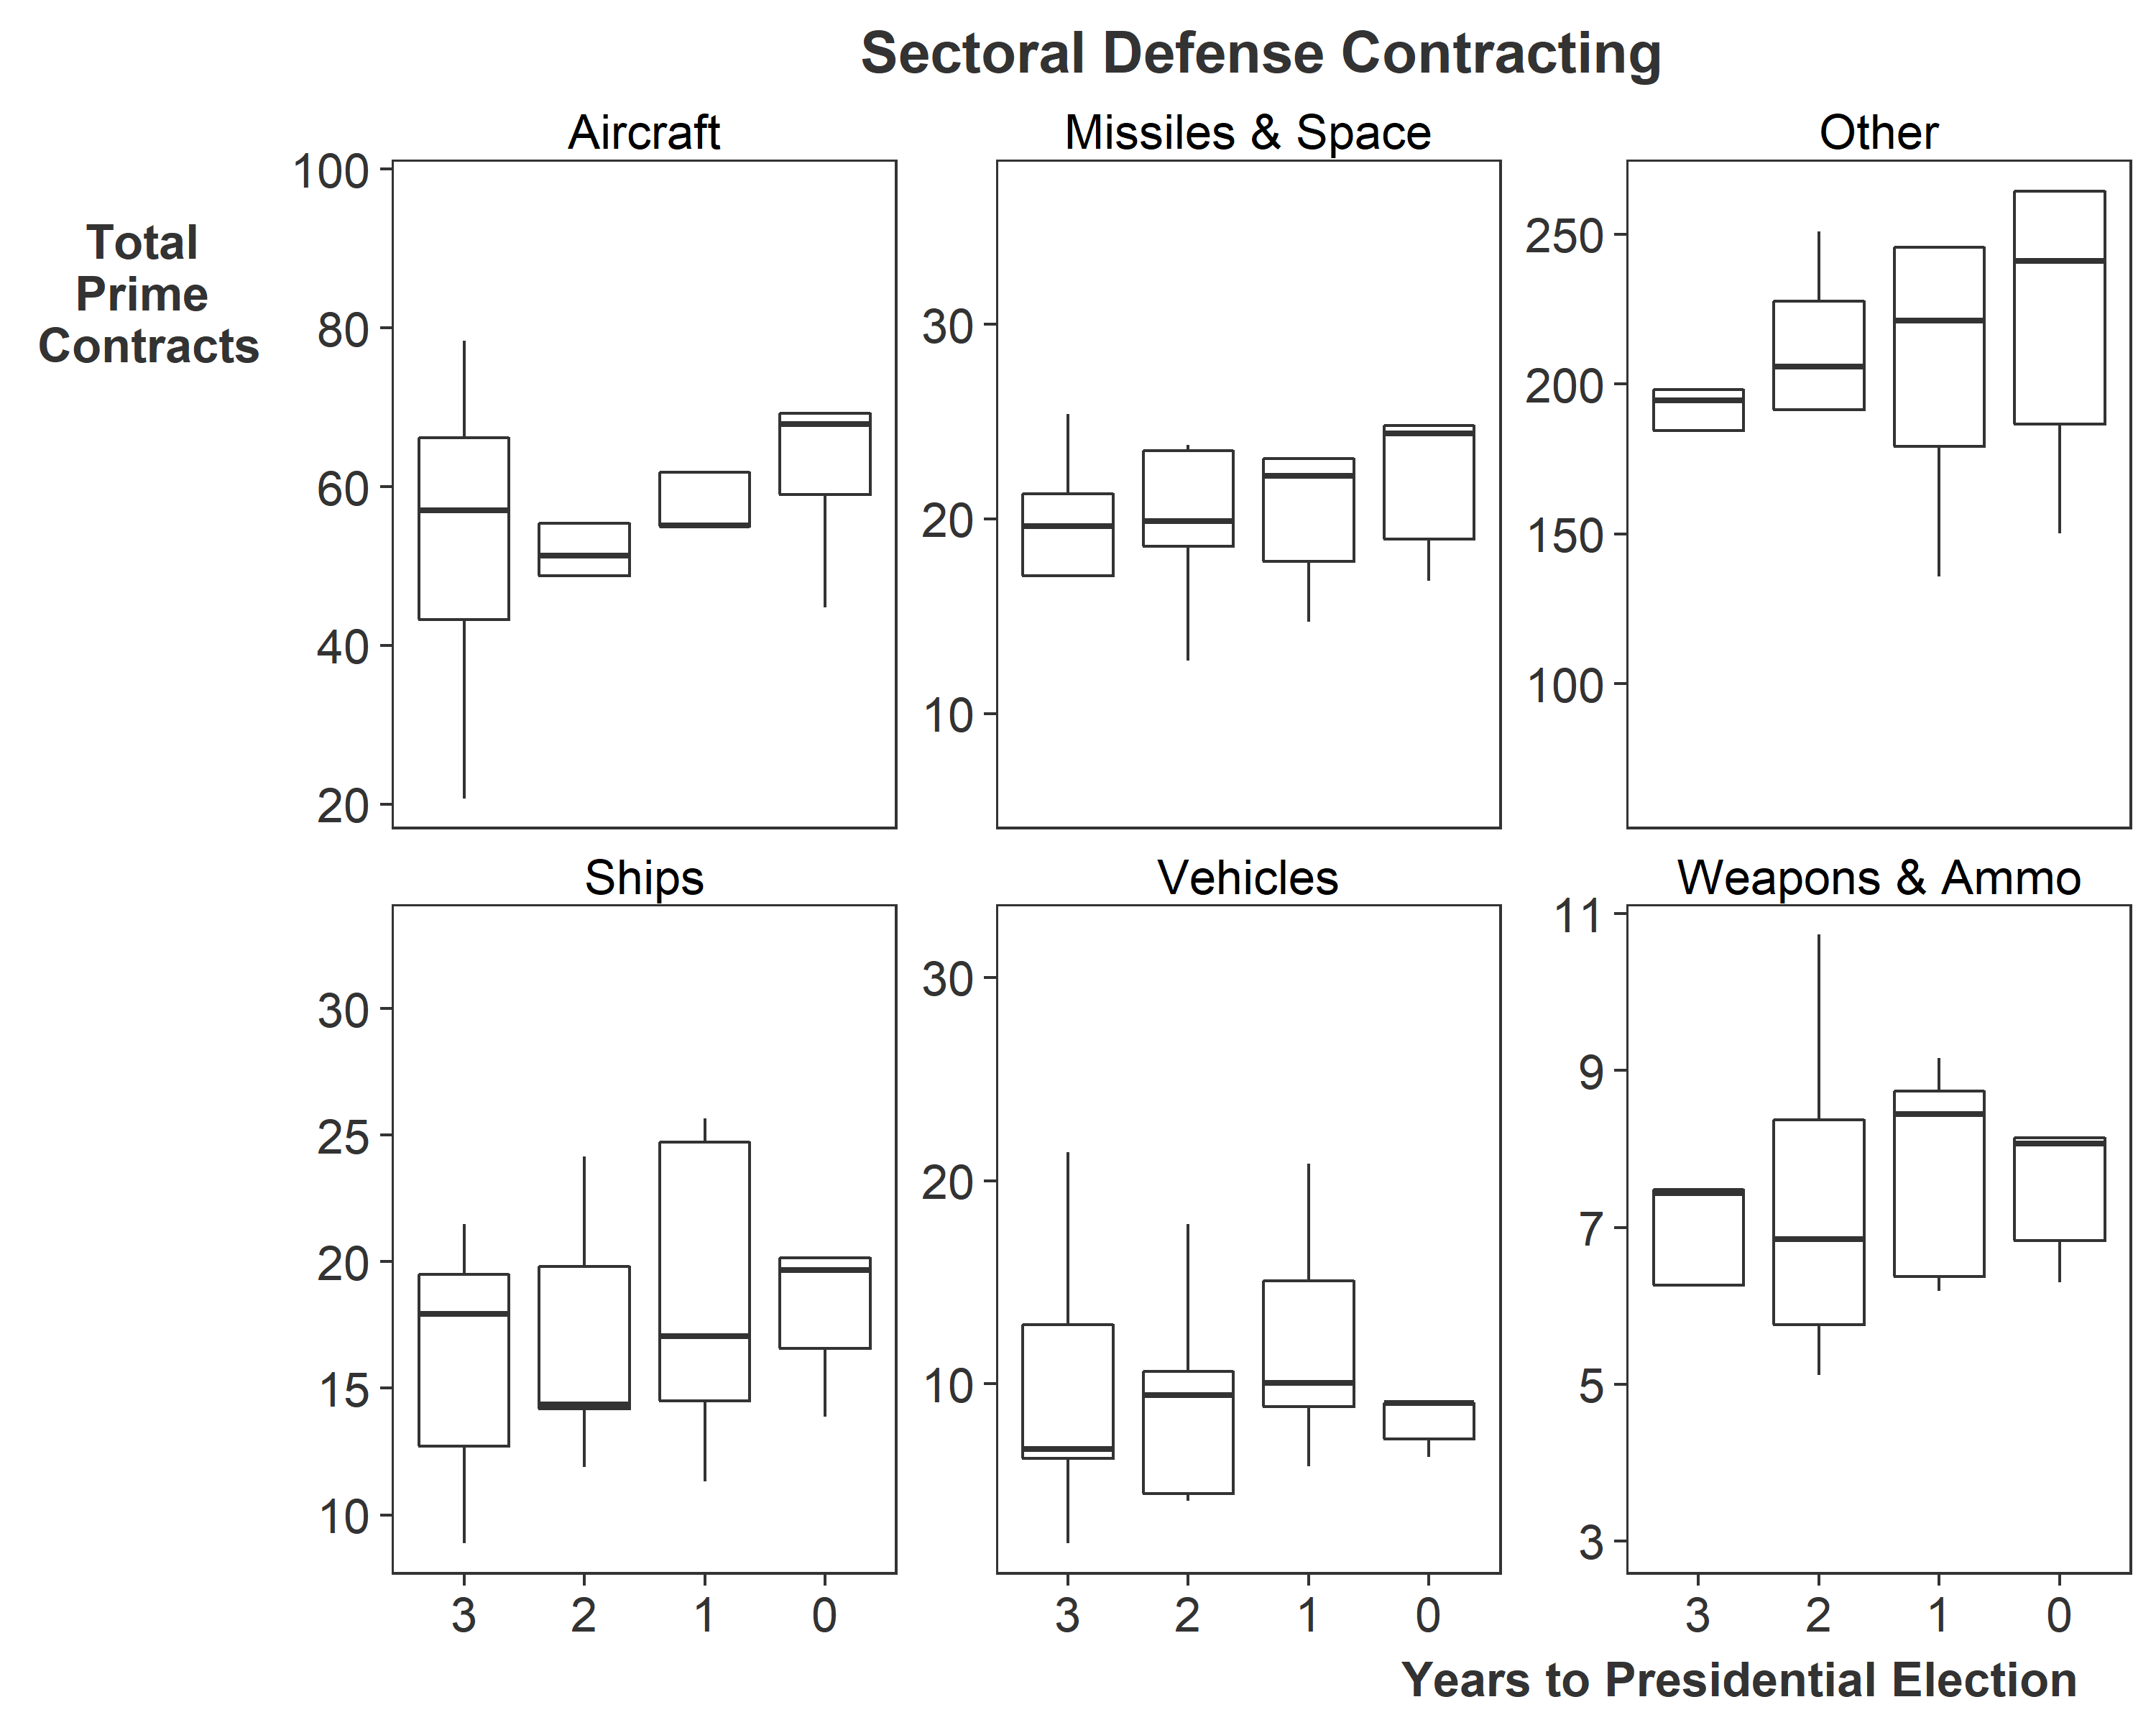
\includegraphics[height=.90\textheight]{contract-cycles-sector.png}
\end{figure}


\end{frame}

%-----------------------------------------------




%----------------------------------------------------------------------------------------

\end{document}
